\documentclass[french, 9pt,xcolor={table,dvipsnames},t,aspectratio=169,onlytextwidth,mathserif]{beamer}

\usetheme{PSU}

% \setbeamercovered{still covered={\opaqueness<1->{0}},again covered={\opaqueness<1->{40}}}

\usepackage{booktabs}
\usepackage{amsmath}
\usepackage{units}
\usepackage{mathrsfs} 
\usepackage{babel}
\usepackage{markdown}
\usepackage{hyperref}

\newtheorem*{remark}{Remarque} % Création d'un nouvel environnement "Remarque"

% Contenu de la page de garde
\title[Stage ČVUT]{Étude théorique : stations de base du réseau téléphonique français}
\subtitle{Progression du stage}
\author{Paul MÉHAUD, Brendan SÉVELLEC}
\institute{České Vysoké Učení Technické v Praze}
\date{mai - août 2024}

\begin{document}

\begin{frame}
  \titlepage
\end{frame}


\begin{frame}{Déroulé de la présentation}
    \tableofcontents
\end{frame}
\addtocontents{toc}{\protect\setcounter{tocdepth}{1}}


\section{Introduction}
\insertsectionframe


\begin{frame}{Contexte général}

    \begin{alertblock}{Objectifs}
        \begin{itemize}
            \item Déterminer si les stations de base sont en zone urbaine ou rurale;
            \item Chercher les stations de bases voisines les unes des autres pour aider à déterminer si les utilisateurs sont en mouvement.
        \end{itemize}
    \end{alertblock}

    \begin{block}{Méthodes}
        \begin{itemize}
            \item Approche par la théorie des graphes ;
            \item Approche par le machine learning.
        \end{itemize}
    \end{block}
\end{frame}


\section{Données}
\insertsectionframe

\begin{frame}{Données}
    \begin{block}{Arcep}
        Autorité de régulation des communications électroniques, des postes et de la distribution de la presse.
    \end{block}

    \begin{block}{Jeu de données}
        Le jeu de données \texttt{2023\_T4\_sites\_Metropole.csv} \footnote{\url{https://data.arcep.fr/mobile/sites/}} représente les stations de bases au trimestre 4 de 2023 avec leur position géographique (taille : $\unit[16,7]{Mo}$).
    \end{block}

    A retenir :
    \begin{itemize}
        \item $108\,838$ sites;
        \item $29$ attributs.
    \end{itemize}
\end{frame}

{
\smallframetitle
\begin{frame}{A quoi ressemble notre base ?}
    \begin{table}[H]
        \centering
        \tiny
        \begin{tabular}{cccccccccc}
        \hline
            \textbf{code\_op} & \textbf{nom\_op} & \textbf{num\_site} & \textbf{id\_site\_partage} & \textbf{id\_station\_anfr} & \textbf{x} & \textbf{y} & \textbf{latitude} & \textbf{longitude} & \textbf{nom\_reg} \\ \hline
            20801 & Orange & 00000001A1 & nan & 0802290015 & 687035 & 6985761 & 49,97028 & 2,81944 & Hauts-de-France \\ 
            20801 & Orange & 00000001B1 & nan & 0642290151 & 422853 & 6249263 & 43,28861 & -0,41389 & Nouvelle-Aquitaine \\ 
            20801 & Orange & 00000001B2 & nan & 0332290026 & 416932 & 6422196 & 44,84112 & -0,58333 & Nouvelle-Aquitaine \\ 
            20801 & Orange & 00000001B3 & nan & 0472290005 & 511106 & 6349234 & 44,21666 & 0,63556 & Nouvelle-Aquitaine \\ 
            20801 & Orange & 00000001C1 & nan & 0512290147 & 836824 & 6889450 & 49,09028 & 4,87333 & Grand Est \\ \hline
        \end{tabular}
        \begin{tabular}{cccccccccc}
        \hline
            \textbf{nom\_dep} & \textbf{insee\_dep} & \textbf{nom\_com} & \textbf{insee\_com} & \textbf{site\_2g} & \textbf{site\_3g} & \textbf{site\_4g} & \textbf{site\_5g} & \textbf{mes\_4g\_trim} & \textbf{site\_ZB} \\ \hline
            Somme & 80 & Curlu & 80231 & 1 & 1 & 1 & 0 & 0 & 0 \\ 
            Pyrénées-Atlantiques & 64 & Jurançon & 64284 & 1 & 1 & 1 & 1 & 0 & 0 \\ 
            Gironde & 33 & Bordeaux & 33063 & 1 & 1 & 1 & 1 & 0 & 0 \\ 
            Lot-et-Garonne & 47 & Agen & 47001 & 1 & 1 & 1 & 0 & 0 & 0 \\ 
            Marne & 51 & Sainte-Menehould & 51507 & 1 & 1 & 1 & 0 & 0 & 0 \\ \hline
        \end{tabular}
        \begin{tabular}{cccccc}
        \hline
            \textbf{site\_DCC} & \textbf{site\_strategique} & \textbf{site\_capa\_240mbps} & \textbf{date\_ouverturecommerciale\_5g} & \textbf{site\_5g\_700\_m\_hz} & \textbf{site\_5g\_800\_m\_hz} \\ \hline
            0 & 0 & 0 & nan & 0 & 0 \\ 
            0 & 0 & 1 & 2020-12-14 & 0 & 0 \\ 
            0 & 0 & 1 & 2021-02-22 & 0 & 0 \\ 
            0 & 0 & 1 & nan & 0 & 0 \\ 
            0 & 0 & 1 & nan & 0 & 0 \\ \hline
        \end{tabular}
        \begin{tabular}{ccc}
        \hline
            \textbf{site\_5g\_1800\_m\_hz} & \textbf{site\_5g\_2100\_m\_hz} & \textbf{site\_5g\_3500\_m\_hz} \\ \hline
            0 & 0 & 0 \\ 
            0 & 1 & 0 \\ 
            0 & 0 & 1 \\ 
            0 & 0 & 0 \\ 
            0 & 0 & 0 \\ \hline
        \end{tabular}
        \caption{Premières valeurs de la base}
    \end{table}
\end{frame}

\begin{frame}{Description (1/2)}
    \begin{block}{Ce qui nous intéresse}
        \begin{enumerate}
            \item \textsl{longitude}, \textsl{latitude} : coordonnées de chaque site;
            \item \textsl{nom\_op} : nom commercial de l'opérateur;
            \item \textsl{nom\_reg}, \textsl{nom\_dep} et \textsl{nom\_com} : nom de la région, du département et de la commune d'implantation du site;
            \item \textsl{site\_$x$g} : équipement du site en technologie $x$G ($x\in\{ 2,\dots,5\}$);
            \item \textsl{num\_site} : identifiant du site issu du SI de l'opérateur. 
        \end{enumerate}
    \end{block}
\end{frame}

\begin{frame}{Description (2/2)}
    \begin{block}{Ce qu'il faut retenir}
        \begin{enumerate}
            \item  Répartition équitable du nombre de sites en fonction de l'opérateur ($\simeq 27\,000$) ;
            \item $99,6\%$ des sites équipés en 4G;
            \item $6$ stations en moyenne par commune.
        \end{enumerate}
    \end{block}

    La construction de cette base ne nous permet pas de faire de statistiques descriptives intéressantes.
\end{frame}
}


\section{Semaine du 07/05/24 au 14/05/24}
\insertsectionframe
\subsection{Brendan}
\insertsubsectionframe

{
\smallframetitle
\subsubsection{Affichages}
\begin{frame}{Affichage des données sur une carte}
    \begin{block}{Détail}
        \begin{itemize}
            \item Découverte d'une bibliothèque d'affichage de données géographiques interactive : \texttt{Folium} ;
            \item Affichage des données et colorisation selon plusieurs critères : technologies (2G, 3G, \dots) ou opérateurs (Free, SFR, Bouygues Telecom ou Orange).
        \end{itemize}
    \end{block}

    \begin{alertblock}{Problème}
        Le nombre de données à afficher est très important et rend la visualisation très saccadée.
    \end{alertblock}

    \begin{block}{Solution}
        Afficher seulement une partie des données à la fois selon différent critères de sélection : par opérateurs, technologie ou région.
    \end{block}
\end{frame}



\begin{frame}{}
    \begin{figure}
        \includegraphics[width=0.7\textwidth]{images/France-Opérateurs.png}
        \caption{\label{fig:fr-op}Les opérateurs dans toute la France}
    \end{figure}
\end{frame}

\begin{frame}{}
    \begin{figure}
        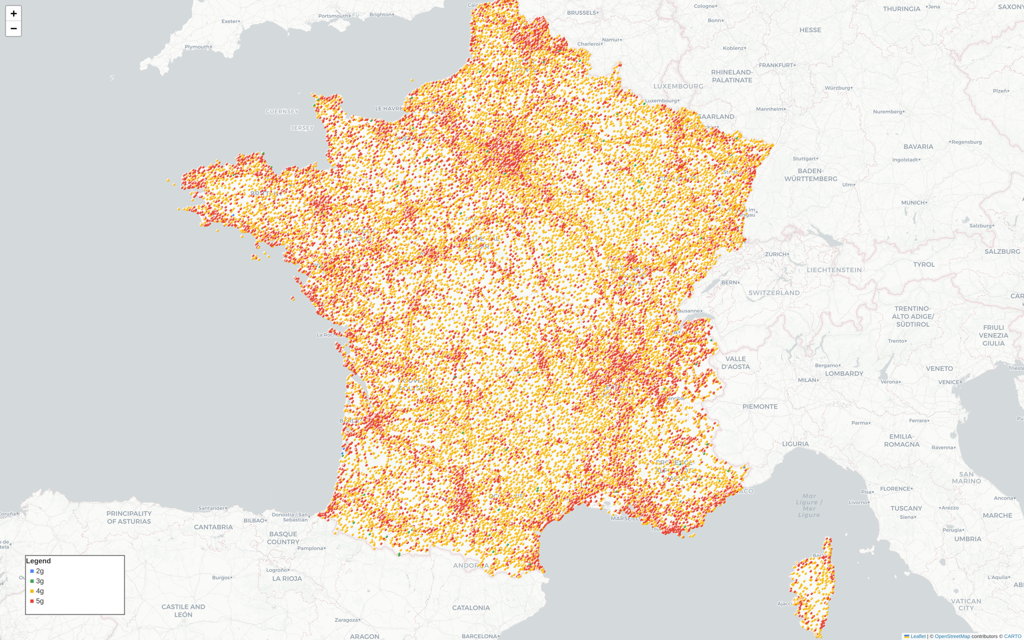
\includegraphics[width=0.7\textwidth]{images/France-Technologies.png}
        \caption{\label{fig:fr-tech}Les technologies dans toute la France}
    \end{figure}
\end{frame}

\begin{frame}{}
    \begin{figure}
        \includegraphics[width=0.7\textwidth]{images/Normandie-Opérateurs.png}
        \caption{\label{fig:no-op}Les opérateurs en Normandie}
    \end{figure}
\end{frame}

\begin{frame}{}
    \begin{figure}
        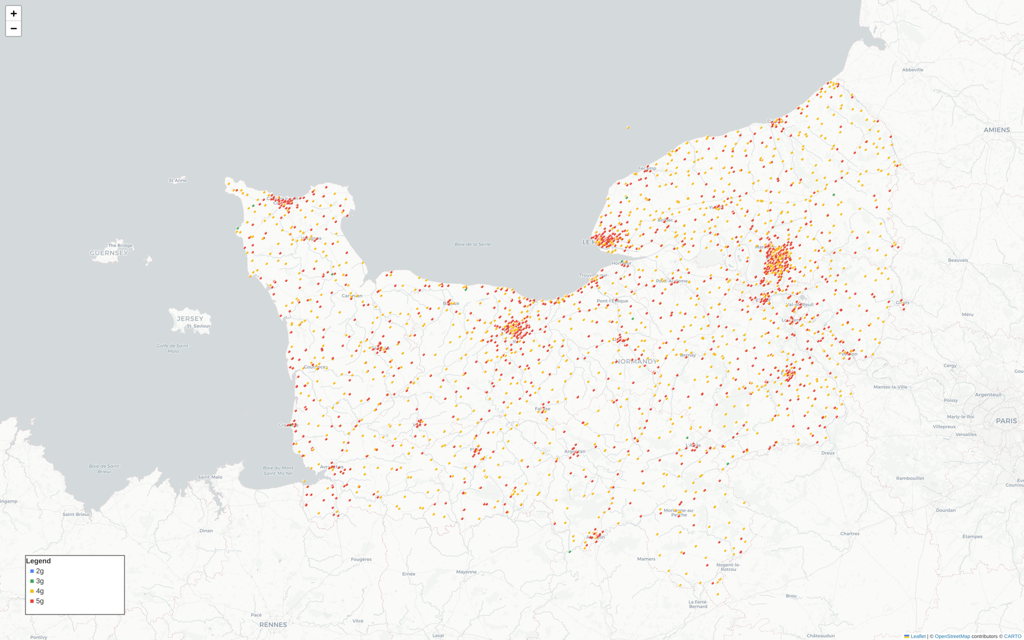
\includegraphics[width=0.7\textwidth]{images/Normandie-Technologies.png}
        \caption{\label{fig:no-tech}Les technologies en Normandie}
    \end{figure}
\end{frame}

\subsubsection{DBScan}
\begin{frame}{Détection des villes}
    Il est très clair que les stations de bases sont très regroupé au sein des villes. Il semble donc qu'il soit possible de détecter si les stations de bases sont en zone rurale ou urbaine à l'aide de la densité de stations de base

    \begin{block}{DBscan (1996)}
        L'algorithme DBscan (Density-Based spatial clustering of applications with noise) est un algorithme qui s'appuie sur la densité estimée des clusters pour effectuer le partitionnement.
    \end{block}
    \begin{block}{Paramètres}
        \begin{itemize}
            \item $\varepsilon$ : dissimilarité maximum entre deux individus ;
            \item $n_{\min}$ : cardinal minimum de chaque classe.
        \end{itemize}
    \end{block}
\end{frame}

\begin{frame}{Théorie : l'algorithme}
    \begin{block}{}
        \begin{enumerate}
            \item Pour chaque point $p_{j}$ :
                \begin{align*}
                    N\left(p_{i}\right) & \gets\left\{ p_{j}, j\in N=\left\{ 1, \dots, n\right\} \mid d(i,j)\leqslant\varepsilon\right\} \\
                    C & \gets\left\{ p_{i}\mid\left|N\left(p_{i}\right)\right|\geqslant n_{\min}\right\} 
                \end{align*}
            \item Construire le graphe de voisinage $G=\left(X, U\right)$, avec $$X=\left\{ p_{i}\mid i\in N\right\} \text{ et } U=\left\{ ij\mid i, j\in N,d(i,j)\leqslant\varepsilon\right\}$$
            \item Trouver les composantes connexes des sommets de $G$ (notées $G_{1}, \dots, G_{p}$) ;
            \item Pour chaque $p_{i}\notin C$ :
                \begin{align*}
                    j^{*} & =\arg\min_{1, \dots, p}\left(d\left(p_{i}, C_{k}\right)\right)\\
                    \text{si } & d\left(p_{i}, C_{j^{*}}\right)\leqslant\varepsilon\text{ alors}\\
                     & C_{j^{*}}\gets C_{j^{*}}\cup\left\{ p_{i}\right\} 
                \end{align*}
        \end{enumerate}
    \end{block}    
\end{frame}

\begin{frame}{}
    \begin{figure}
        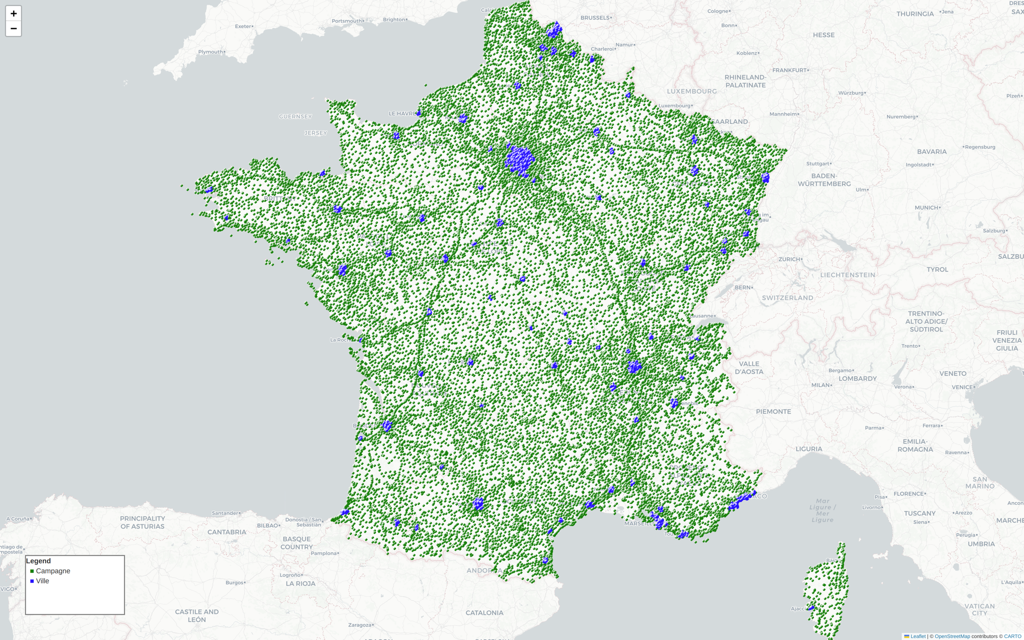
\includegraphics[width=0.7\textwidth]{images/France-Villes-Orange_0.03_15.png}
        \caption{\label{fig:fr-vi-or-0.03-15}Les villes détectées en France pour l'opérateur Orange avec $\epsilon=0.03$ et $n_{min}=15$}
    \end{figure}
\end{frame}


\subsubsection{Delaunay et Voronoï}

\begin{frame}{Diagramme de Voronoï}
    \begin{columns}
        \begin{column}{0.6\textwidth}
            \begin{block}{Définition}
                Le diagramme de Voronoï associé à un ensemble de points $(d_i)_{1\leq i \leq n}$ est un pavage de l'espace tel que chaque pavé $P_i$ représente l'ensemble des points plus proches de $d_i$ que de n'importe quel $d_j$ avec $j\neq i$ i.e.
            \end{block}
        \end{column}
            
        \begin{column}{0.4\textwidth}
            \begin{figure}
                
\includegraphics[width=0.5\textwidth]{images/Coloured_Voronoi_2D.png}
                \caption{\label{fig:vor-ex}Exemple de diagramme de Voronoï}
            \end{figure}
        \end{column}
    \end{columns}
    
            
\end{frame}

\begin{frame}{Triangulation de Delaunay}
    \begin{columns}
        \begin{column}{0.6\textwidth}
            \begin{block}{Définition}
                La triangulation de Delaunay d'un ensemble $P$ de points du plan est une triangulation $DT(P)$ telle qu'aucun point de $P$ n'est à l'intérieur du cercle circonscrit d'un des triangles de $DT(P)$. Les triangulations de Delaunay maximisent le plus petit angle de l'ensemble des angles des triangles, évitant ainsi les triangles \og allongés \fg{}.
            \end{block}
        \end{column}
            
        \begin{column}{0.4\textwidth}
             \begin{figure}
                
\includegraphics[width=0.5\textwidth]{images/Delaunay_circumcircles_vectorial.svg.png}
                \caption{\label{fig:del-ex}Exemple de triangulation de Delaunay}
            \end{figure}
        \end{column}
    \end{columns}
\end{frame}

\begin{frame}{Lien entre les 2}
    \begin{columns}
        \begin{column}{0.6\textwidth}
            \begin{block}{Propriétés}
                \begin{itemize}
                    \item La triangulation de Delaunay d’un ensemble discret $P$ de points est le graphe dual du diagramme de Voronoï associé à $P$;
                    \item Il est donc très facile de passer de l'un à l'autre (en temps polynomial);
                    \item il existe des algorithmes pour trouver une triangulation de Delaunay en $O(n\log(n))$.
                \end{itemize}      
            \end{block} 
        \end{column}
            
        \begin{column}{0.4\textwidth}
            \begin{figure}
                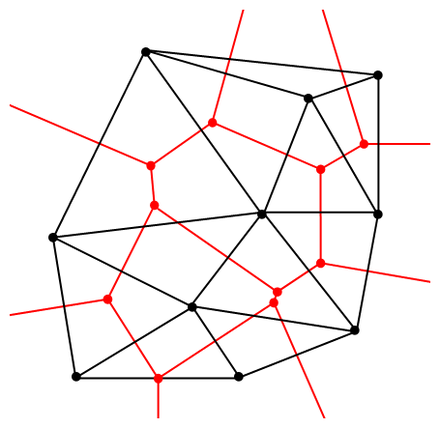
\includegraphics[width=0.5\textwidth]{images/Delaunay_Voronoi.png}
                \caption{\label{fig:del-vor}Lien entre Delaunay et Voronoï}
            \end{figure}
        \end{column}
    \end{columns} 
\end{frame}

\begin{frame}{Retour au problème}
    \begin{block}{Application à notre cas d'étude}
        Nous allons pouvoir utiliser ces notions en définissant :
        \begin{itemize}
            \item les voisins potentiels comme étant les triangles adjacents dans la triangulation de Delaunay
            \item les zones de couverture des antennes comme les pavés associé dans le diagramme de Voronoï
        \end{itemize}
    \end{block}
\end{frame}
}

\subsection{Paul}
\insertsubsectionframe

\begin{frame}{Résumé des épisodes précédents}
    Mon travail, pour la semaine qui vient de s'écouler, s'articule autour de trois axes majeurs :
    \begin{block}{}
        \begin{itemize}
            \item Découverte des données ;
            \item Documentation ;
            \item Reprise du travail de l'année précédente.
        \end{itemize}
    \end{block}
        
\end{frame}

{
\smallframetitle
\begin{frame}{Documentation}
    La majeure partie du travail de la semaine écoulée a consisté à se former aux différents outils de \texttt{Python} afin de pouvoir effectuer sereinement le travail.

    \begin{block}{Outils utilisés}
        \begin{itemize}
            \item \texttt{pandas.DataFrame} : gestion des données ;
            \item \texttt{scipy.spatial.Delaunay} : création de la triangulation de Delaunay ;
            \item \texttt{networkx.Graph} : création de graphes ;
            \item \texttt{matplotlib.pyplot} : affichage des résultats.
        \end{itemize}
    \end{block}
\end{frame}

\begin{frame}{Reprise du travail précédent (1/3)}
    La première tâche consistait à essayer de faire fonctionner le code fourni. Résultat : il ne fonctionne pas\dots
    
    Décision : refaire par moi-même. Cependant, j'ai gardé les idées.
    \begin{block}{Approche pour déterminer les voisins de stations de base}
        \begin{itemize}
            \item Faire une triangulation de Delaunay (liste de voisins potentiels);
            \item Eliminer les voisins distants de plus de $\unit[15]{km}$ ;
            \item Garder le voisin le plus proche dans chaque cadrant autour de chaque station (6 cadrants);
            \item Garder le voisin le plus proche quand deux stations voisines sont séparées par un angle faible.
        \end{itemize}
            
    \end{block}
\end{frame}

\begin{frame}{Reprise du travail précédent (2/3)}
    Ayant refait l'implantation moi-même, j'ai décidé d'utiliser les graphes au lieu de simplement les datasFrames : permettra de faciliter l'application de la théorie des graphes.
    \begin{block}{Apports de cette nouvelle représentation}
        \begin{itemize}
            \item On travail directement sur le graphe de Delaunay ;
            \item Le traitement des voisins est beaucoup plus facile ;
            \item La représentation graphique est plus claire.
        \end{itemize}
    \end{block}
\end{frame}

\begin{frame}{Reprise du travail précédent (3/3) : Résultats}
    Pour l'instant seul les deux premiers critères de filtrage sont fonctionnels. Voici ce que l'on obtient sur le département du Gard :
    \begin{figure}
        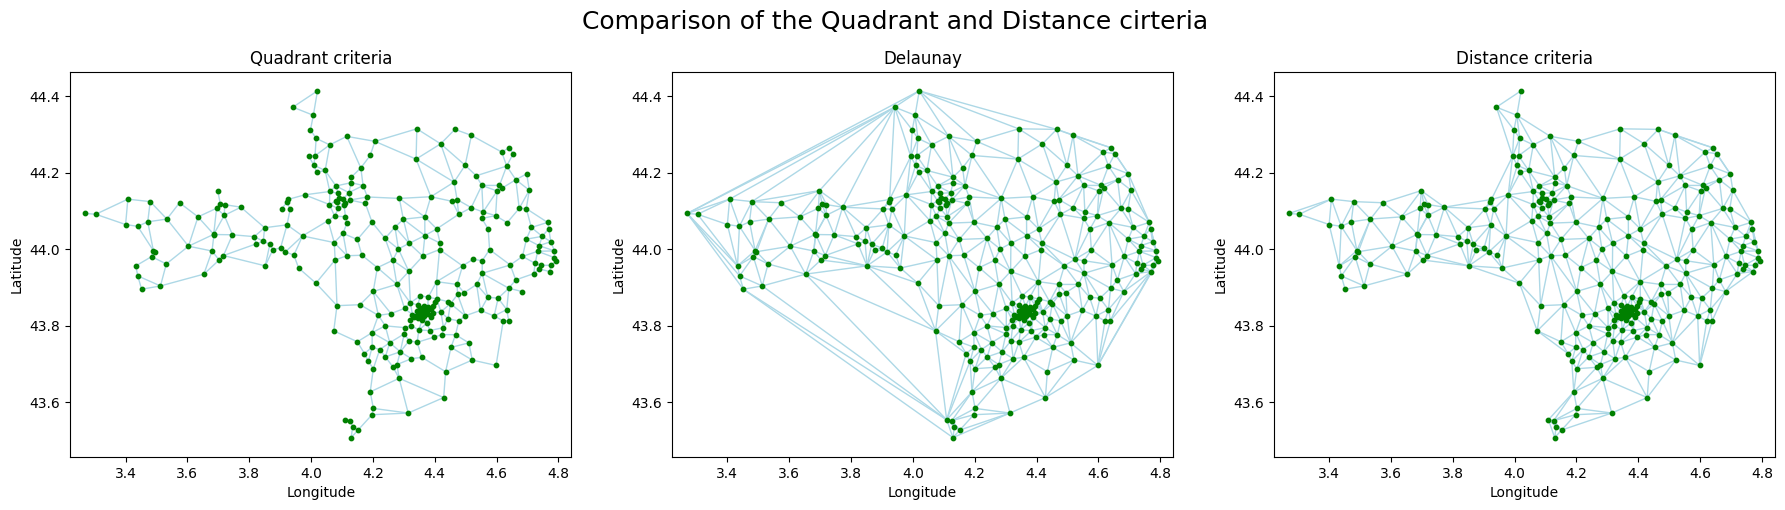
\includegraphics[width=0.9\textwidth]{images/comparaison_criteres.png}
        \caption{\label{fig:comp-crit}Evolution de la triangulation de Delaunay en fonction de critères de filtrage}
    \end{figure}
\end{frame}

\begin{frame}{Perspectives d'amélioration et travail à venir}
    \begin{block}{Améliorations}
        \begin{itemize} 
            \item Vérifier que l'algorithme du critère du quadrant donne les bons résultats;
            \item Optimisation dudit algorithme.
        \end{itemize}
    \end{block}

    \begin{block}{Travail à venir}
        \begin{itemize} 
            \item Implanter une version fonctionnelle du critère de l'angle;
            \item Se renseigner sur l'état de l'art de la théorie des graphes.
        \end{itemize}
    \end{block}
\end{frame}
}




\subsection{Brendan}
\insertsubsectionframe
\begin{frame}{Réalisation d'une interface graphique en \texttt{Python}}
    \begin{block}{Contexte}
        \begin{itemize}
            \item Beaucoup de cartes à tracer car beaucoup de paramètres ;
            \item Cartes gourmandes en ressources et pas adaptées à des notebooks \texttt{Python} ;
            \item Réalisation d'une application permettant de facilement tracer ces cartes au sein d'un navigateur web.
        \end{itemize}
    \end{block}
    
\end{frame}

\smallframetitle

\section{Semaine du 14/05/24 au 21/05/24}
\insertsectionframe
\subsection{Le jeu de donnée}
\insertsubsectionframe

\begin{frame}{Le jeu de donnée}
    \begin{block}{Arcep}
        L'autorité de régulation des communications électroniques, des postes et de la distribution de la presse (Arcep) est une autorité administrative indépendante française chargée de réguler les communications électroniques et postales et la distribution de la presse.
    \end{block}

    \begin{block}{Mon Réseau Mobile}
        Mon Réseau Mobile est la plate-forme cartographique regroupant l’ensemble des données géographiques en lien avec les réseaux dits \og mobiles \fg{} (2G, 3G, 4G, 5G) régulés par l’Arcep.
    \end{block}

    \begin{alertblock}{Nouvelle mise à jour}
        Une nouvelle mise à jour des données est prévue de \textbf{jeudi 20 juin 2024} à 17h40 : données du 1\ier{} trimestre de 2024.
    \end{alertblock}

    A cette adresse : \url{https://www.data.gouv.fr/fr/datasets/mon-reseau-mobile/\#/discussions}, on peut poser nos questions sur le jeu de données.
\end{frame}


\begin{frame}{Arborescence du jeu de données}
    \begin{columns}
        \begin{column}{0.4\textwidth}
            Les fichiers de données sont rangés par trimestre de publication, zone (France métropolitaine/Outre-mer) et département le cas échéant :
        \end{column}
            
        \begin{column}{0.6\textwidth}
            \begin{figure}
                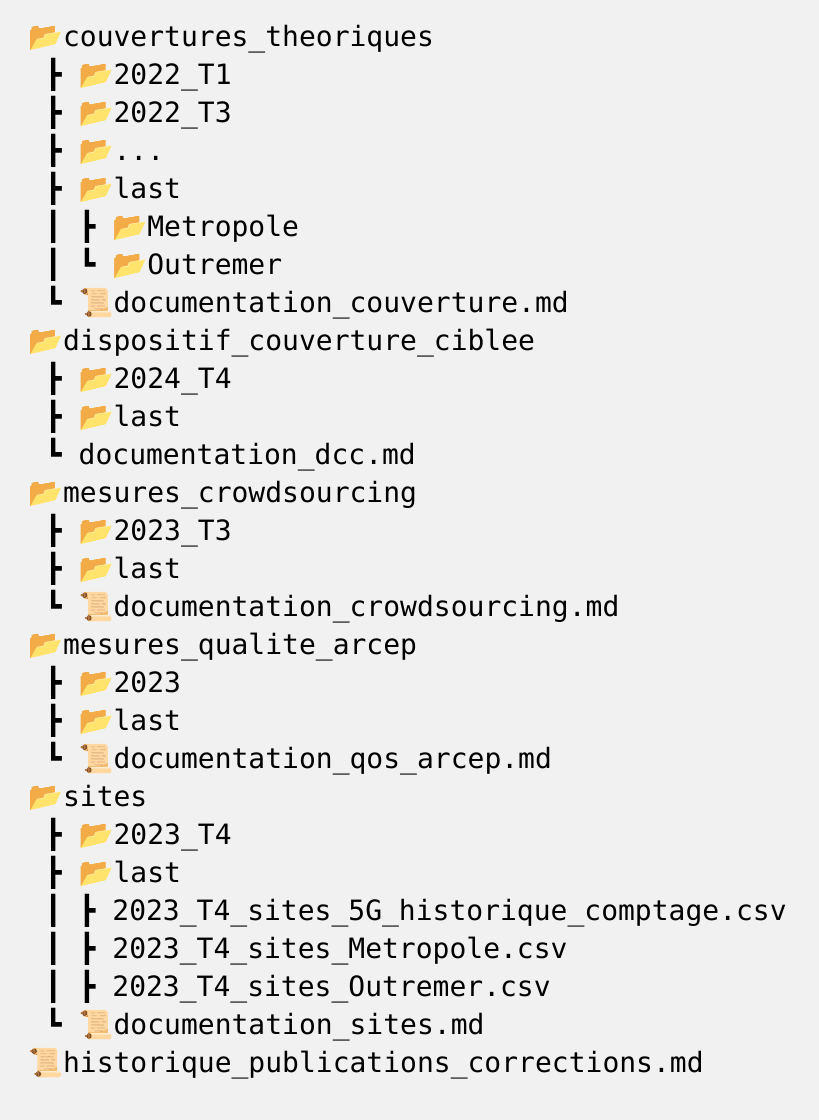
\includegraphics[height=0.55\paperheight]{images/architecture.png}
                \caption{\label{fig:archi}Architecture de la base de donnée}
            \end{figure}
        \end{column}
    \end{columns} 
    
\end{frame}

\begin{frame}{Fréquences de mises à jour}
    \begin{figure}
        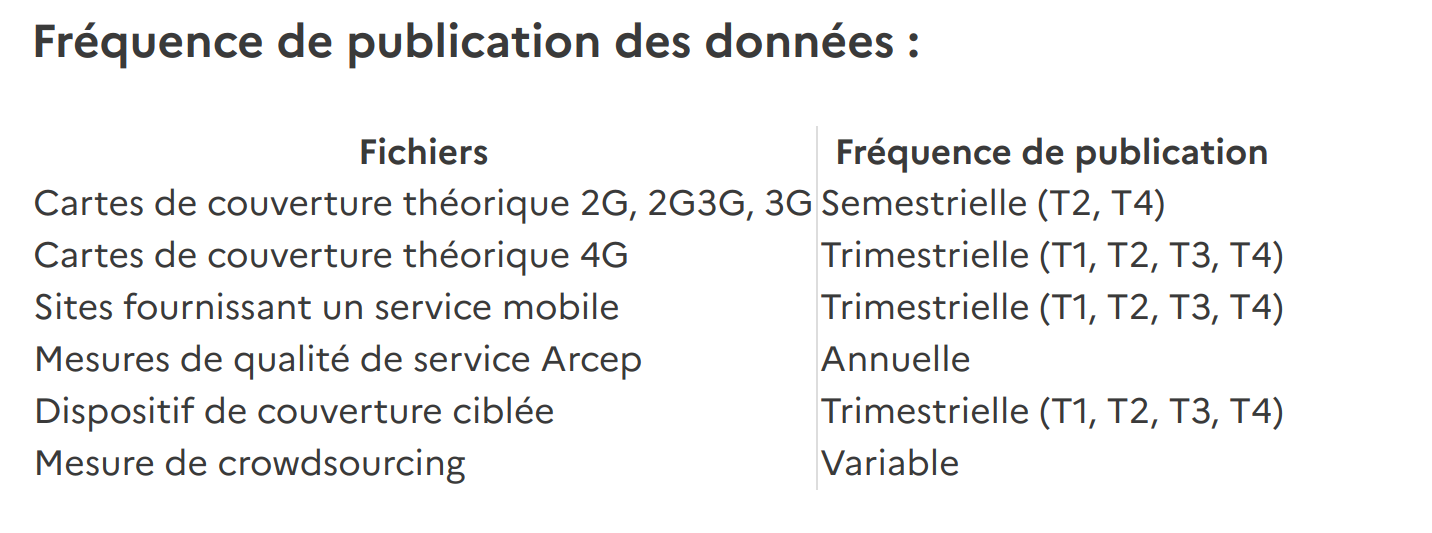
\includegraphics[height=0.5\paperheight]{images/frequence.png}
        \caption{\label{fig:freq}Fréquence de publication de mises à jour}
    \end{figure}
\end{frame}


\subsection{Faisons parler les données}
\insertsubsectionframe

\begin{frame}{Quelques chiffres en vrac}
    Tout d'abord, remarquons que chaque station peut être identifiée à son \texttt{num\_site} (seul deux stations n'en n'ont pas).
    Ensuite, voici ce que l'on a découvert :
    \begin{block}{Des chiffres sympathiques}
        \begin{itemize}
            \item \texttt{site\_zb} : $10\,596$ (Site issu du programme \og zones blanches – centres-bourgs\fg{}) ;
            \item \texttt{site\_dcc} : $10\,627$ (Site issu du \og Dispositif de Couverture Ciblée\fg{}) ;
            \item \texttt{site\_strategique} : $144$ (Site issu du programme \og France Mobile\fg{}) ;
            \item \texttt{mes\_4g\_trim} : $1\,618$ (Equipement du site en technologie 4g au cours du dernier trimestre (du 30/06/2022 au 30/09/2022)) ;
            \item \texttt{id\_site\_partage} : $5\,453$ (Sites mutualisés entre plusieurs opérateurs) ;
            \item \texttt{site\_capa\_204mbps} : $92\,664$ (Site dont la capacité maximum théorique est supérieure ou égale à $\unit[240]{Mbs}$).
        \end{itemize}
    \end{block}
\end{frame}

\begin{frame}{Quelques chiffres en vrac : précision sur les indicateurs}
    Ensuite, voici ce que l'on a découvert :
    \begin{block}{\texttt{site\_zb}}
        Le premier programme, initié en 2003 et nommé \og zones blanches – centres-bourgs\fg{} consistait à apporter des services de téléphonie mobile, SMS et internet mobile à très haut débit, dans plus de 3500 centres-bourgs de communes de France qui ne bénéficiaient d’aucune couverture mobile.
        \footnotemark[1]
    \end{block}

    \begin{block}{\texttt{site\_dcc}}
        Le dispositif de couverture ciblée vise à assurer une couverture mobile de qualité dans des zones non ou mal couvertes, en construisant jusqu’à 5 000 nouveaux sites par opérateur, dont une partie sera mutualisée.
        \footnotemark[2]
    \end{block}
    
    \footnotetext[1]{\url{https://www.tactis.fr/zone-blanche-zone-grise/}}
    \footnotetext[2]{\url{https://agence-cohesion-territoires.gouv.fr/france-mobile-54}}
\end{frame}



\begin{frame}{Comparaison des différents équipements en terme de technologies (1/7)}
    Voici tout d'abord un graphique sur la présence d'une technologie en fonction de l'opérateur (une technologie présente sur un site n'exclue pas la présence d'une autre technologie) :
    \begin{figure}
        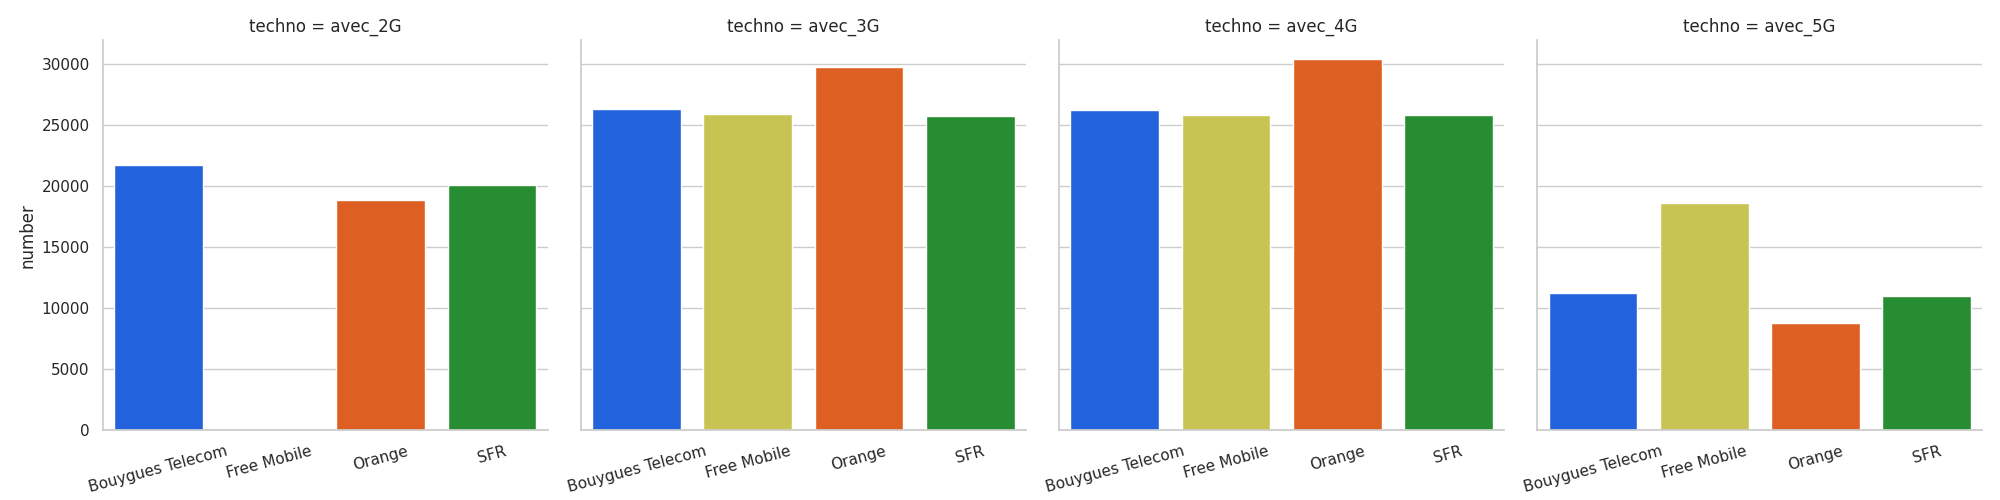
\includegraphics[height=0.4\paperheight]{images/barplots/avec_techno.png}
        \caption{\label{fig:av_tech}Nombres de sites équipés d'au moins une technologie}
    \end{figure}
\end{frame}

\begin{frame}{Comparaison des différents équipements en terme de technologies (2/7)}
    \begin{table}[!ht]
        \centering
        \footnotesize
        \begin{tabular}{cccccc}
        \hline
            \textbf{Technologie} & \textbf{Bouygues Telecom} & \textbf{Free Mobile} & \textbf{Orange} & \textbf{SFR} & \textbf{Total} \\ \hline
            \textbf{2G} & 4 & 0 & 10 & 20 & 34 \\ 
            \textbf{3G} & 30 & 102 & 65 & 37 & 234 \\ 
            \textbf{4G} & 15 & 15 & 602 & 106 & 738 \\ 
            \textbf{5G} & 0 & 0 & 3 & 0 & 3 \\ 
            \textbf{2-3G} & 66 & 0 & 21 & 80 & 167 \\ 
            \textbf{2-4G} & 12 & 0 & 63 & 67 & 142 \\ 
            \textbf{2-5G} & 0 & 0 & 0 & 0 & 0 \\ 
            \textbf{3-4G} & 3889 & 7225 & 9288 & 4909 & 25311 \\ 
            \textbf{3-5G} & 0 & 0 & 0 & 0 & 0 \\ 
            \textbf{4-5G} & 6 & 0 & 109 & 38 & 153 \\ 
            \textbf{2-3-4G} & 11044 & 0 & 11697 & 9831 & 32572 \\ 
            \textbf{2-3-5G} & 0 & 0 & 1 & 0 & 1 \\ 
            \textbf{2-4-5G} & 0 & 0 & 5 & 10 & 15 \\ 
            \textbf{3-4-5G} & 681 & 18607 & 1638 & 835 & 21761 \\ 
            \textbf{2-3-4-5G} & 10584 & 0 & 7038 & 10085 & 27707 \\ 
            \textbf{Total} & 26331 & 25949 & 30540 & 26018 & 108838 \\ \hline
        \end{tabular}
        \caption{Résumé des données de présence de technologie}
    \end{table}
\end{frame}

\begin{frame}{Comparaison des différents équipements en terme de technologies (3/7)}
    Maintenant nous nous intéressons à la fréquence de présence de certaines technologies et pas d'autres :
    \begin{figure}
        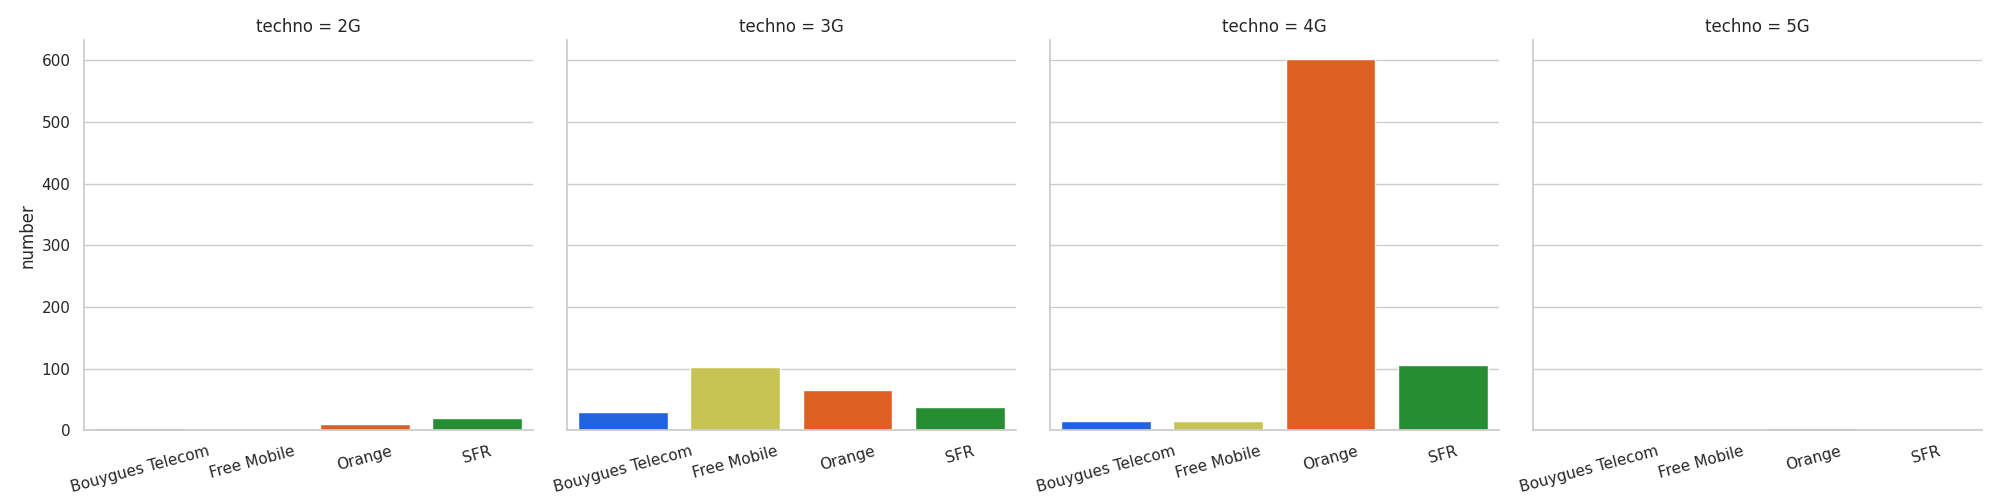
\includegraphics[height=0.4\paperheight]{images/barplots/xG.png}
        \caption{\label{fig:xG}Nombres de sites équipés d'une unique technologie}
    \end{figure}
\end{frame}

\begin{frame}{Comparaison des différents équipements en terme de technologies (4/7)}
    \begin{figure}
        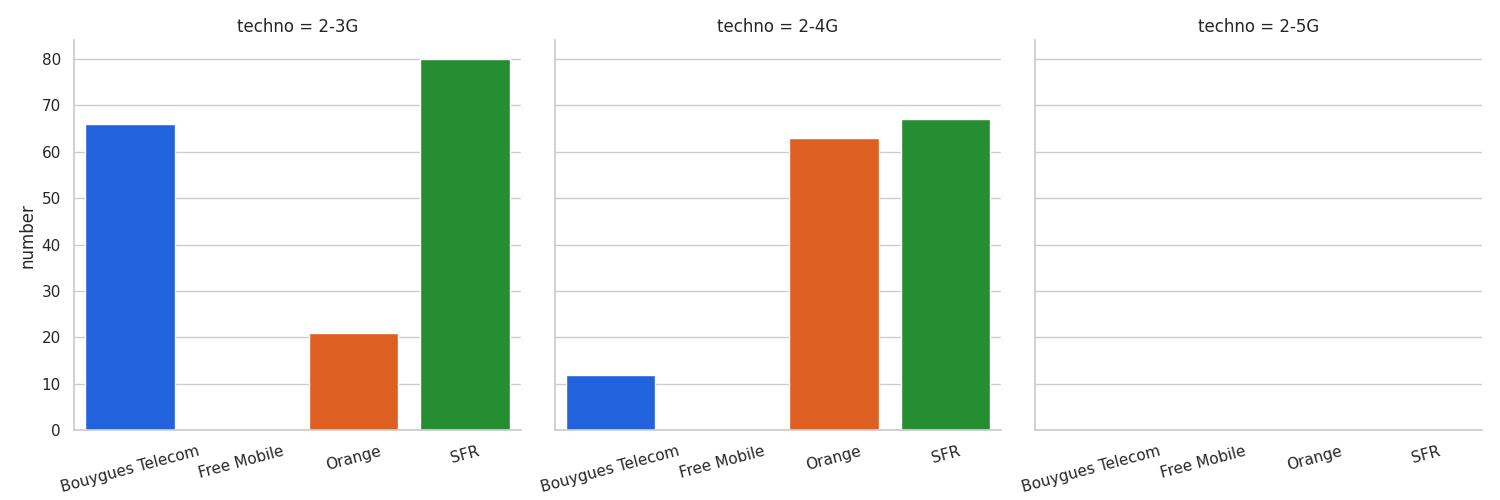
\includegraphics[height=0.4\paperheight]{images/barplots/2-xG.png}
        \caption{\label{fig:2-xG}Nombres de sites équipés de deux technologies}
    \end{figure}
\end{frame}

\begin{frame}{Comparaison des différents équipements en terme de technologies (5/7)}
    \begin{columns}
        \begin{column}{0.65\textwidth}
            \begin{figure}
                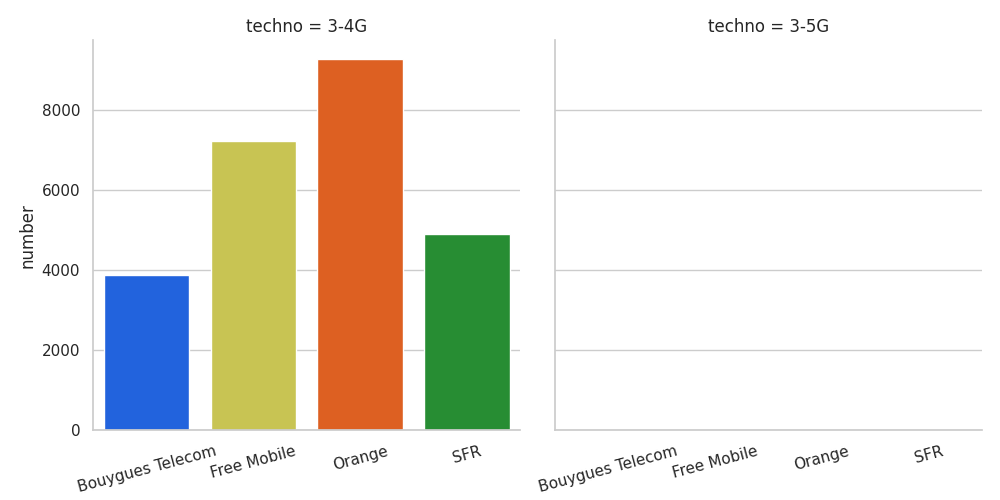
\includegraphics[height=0.4\paperheight]{images/barplots/3-xG.png}
                \caption{\label{fig:3-xG}Nombres de sites équipés de deux technologies (suite)}
            \end{figure}
        \end{column}
            
        \begin{column}{0.35\textwidth}
            \begin{figure}
                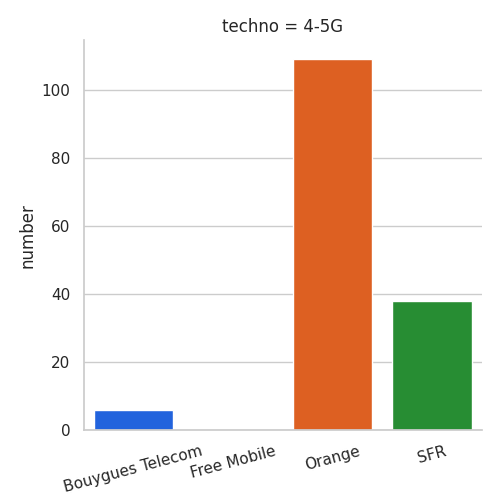
\includegraphics[height=0.4\paperheight]{images/barplots/4-5G.png}
                \caption{\label{fig:4-5G}Nombres de sites équipés de deux technologies (suite-bis)}
            \end{figure}
        \end{column}
    \end{columns} 
\end{frame}

\begin{frame}{Comparaison des différents équipements en terme de technologies (6/7)}
    \begin{figure}
        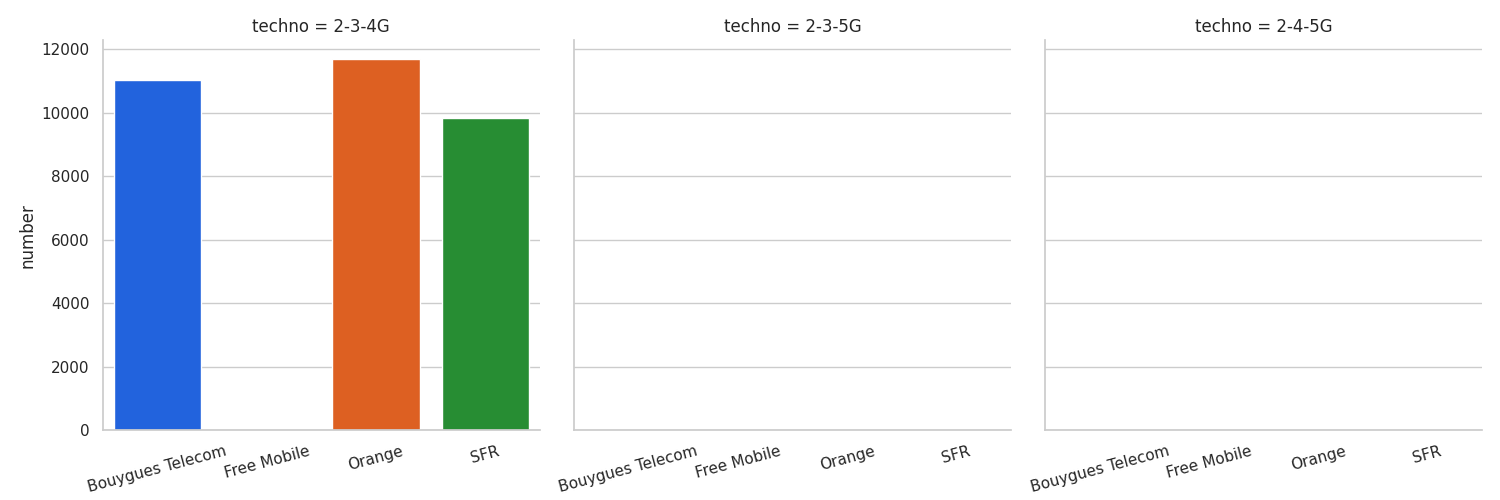
\includegraphics[height=0.4\paperheight]{images/barplots/2-x-yG.png}
        \caption{\label{fig:2-x-yG}Nombres de sites équipés de trois technologies}
    \end{figure}
\end{frame}

\begin{frame}{Comparaison des différents équipements en terme de technologies (7/7)}
    \begin{columns}
        \begin{column}{0.35\textwidth}
            \begin{figure}
                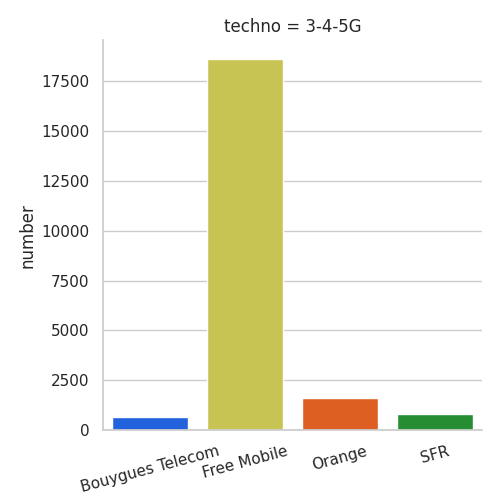
\includegraphics[height=0.4\paperheight]{images/barplots/3-4-5G.png}
                \caption{\label{fig:3-4-5G}Nombres de sites équipés de trois technologies (suite)}
            \end{figure}
        \end{column}
            
        \begin{column}{0.65\textwidth}
            \begin{figure}
                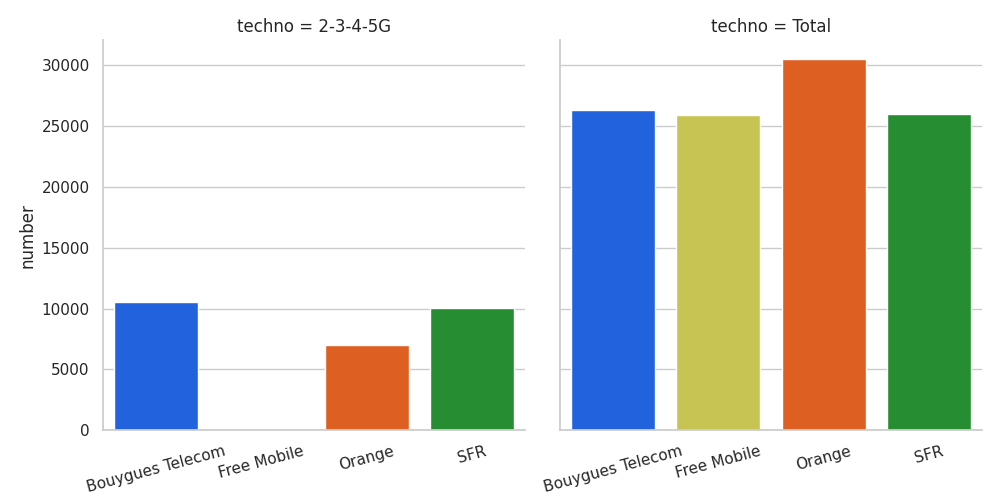
\includegraphics[height=0.4\paperheight]{images/barplots/all-tot.png}
                \caption{\label{fig:all-tot}Nombre de sites équipés de toutes les technologies et total}
            \end{figure}
        \end{column}
    \end{columns} 
\end{frame}

\subsection{Affichage plus détaillé des cartes}
\insertsubsectionframe

\subsubsection{Les stations de base par opérateurs}
\begin{frame}{Les stations de base par opérateur}
    \begin{figure}
        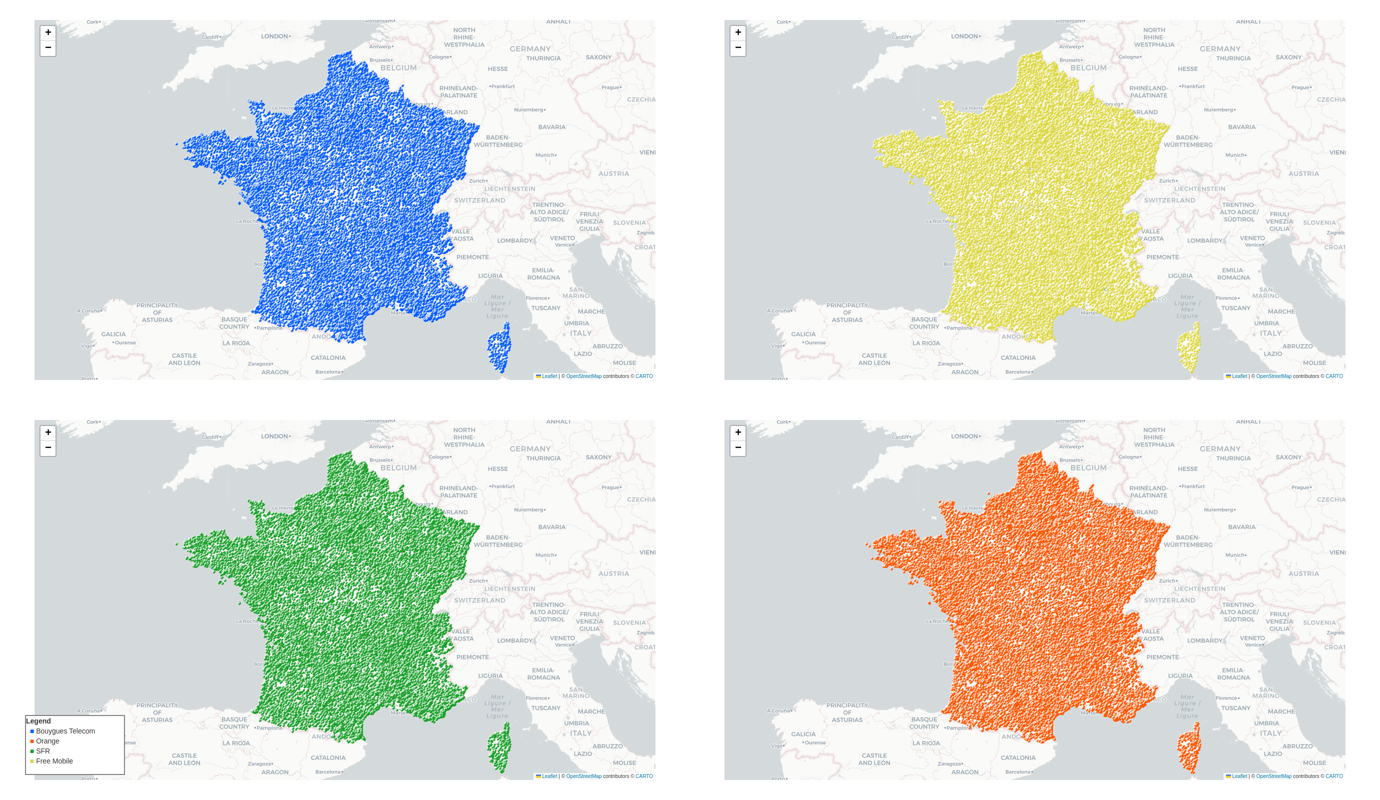
\includegraphics[width=0.9\paperheight]{images/cartes/subplots-providers.png}
        \caption{\label{fig:sp-prov}Les stations de base par opérateurs}
    \end{figure}
\end{frame}


\subsubsection{Les technologies par opérateurs}
\subsubsection{Les technologies par opérateurs}
\begin{frame}{Les stations 2G}
    \begin{figure}
        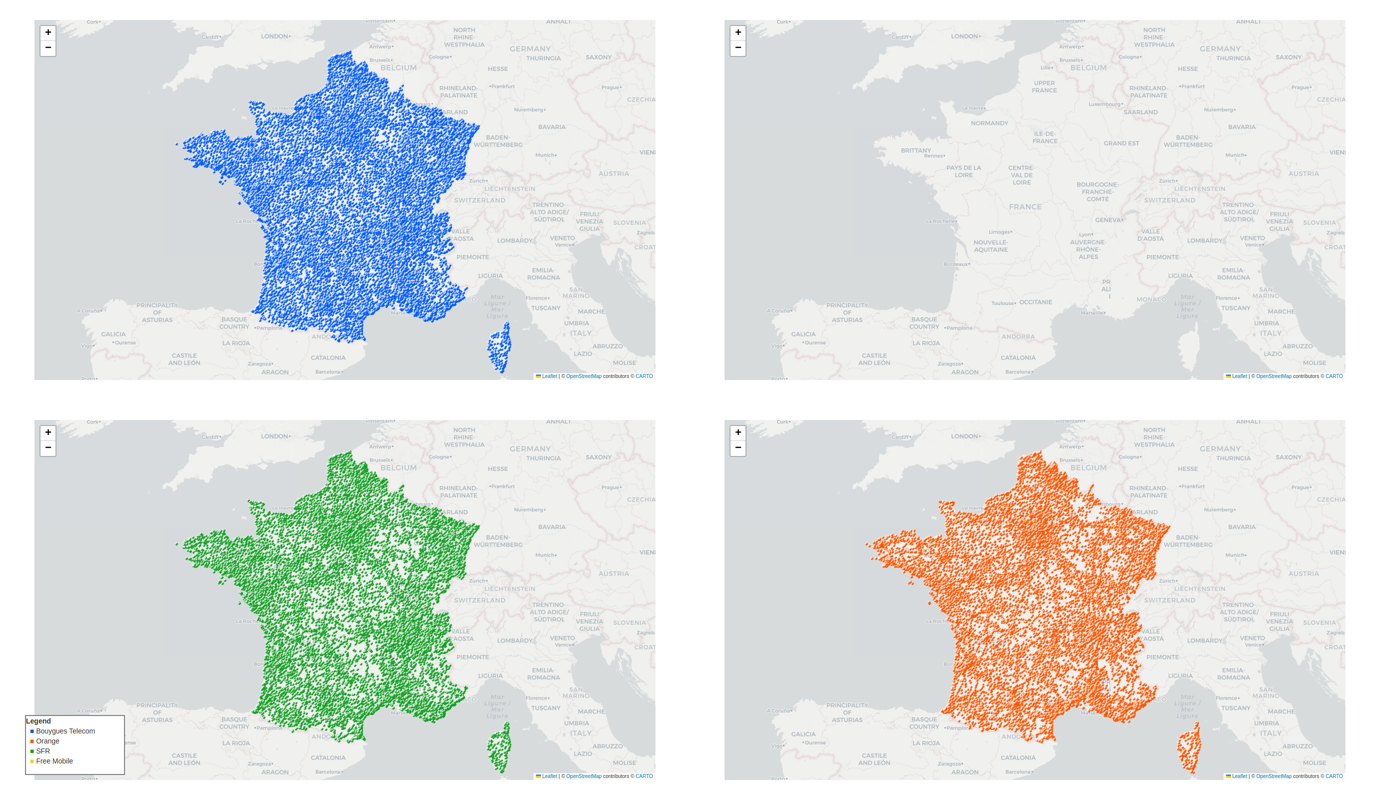
\includegraphics[width=0.9\paperheight]{images/cartes/providers-site_2g.png}
        \caption{\label{fig:sp-2g}Les stations 2G}
    \end{figure}
\end{frame}

\begin{frame}{Les stations 3G}
    \begin{figure}
        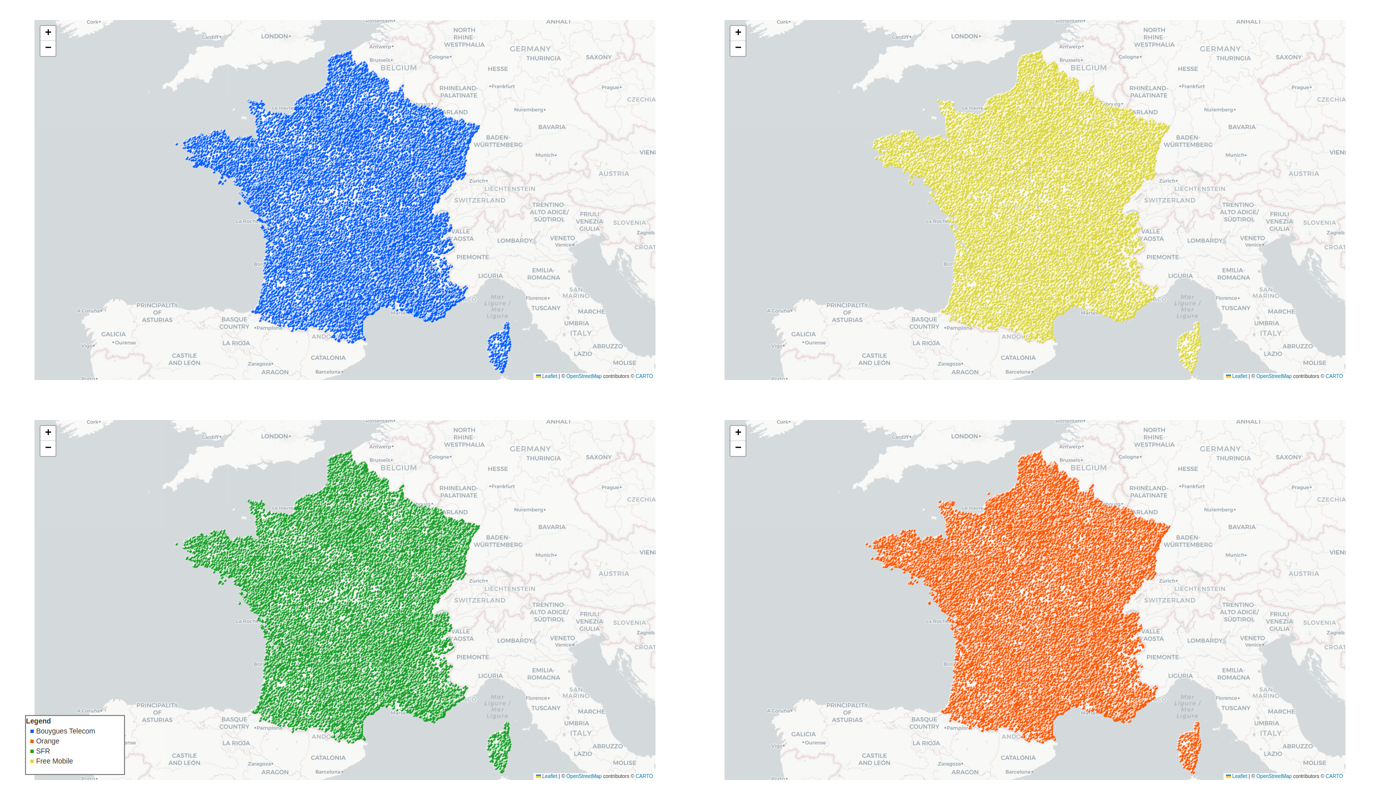
\includegraphics[width=0.9\paperheight]{images/cartes/providers-site_3g.png}
        \caption{\label{fig:sp-3g}Les stations 3G}
    \end{figure}
\end{frame}

\begin{frame}{Les stations 4G}
    \begin{figure}
        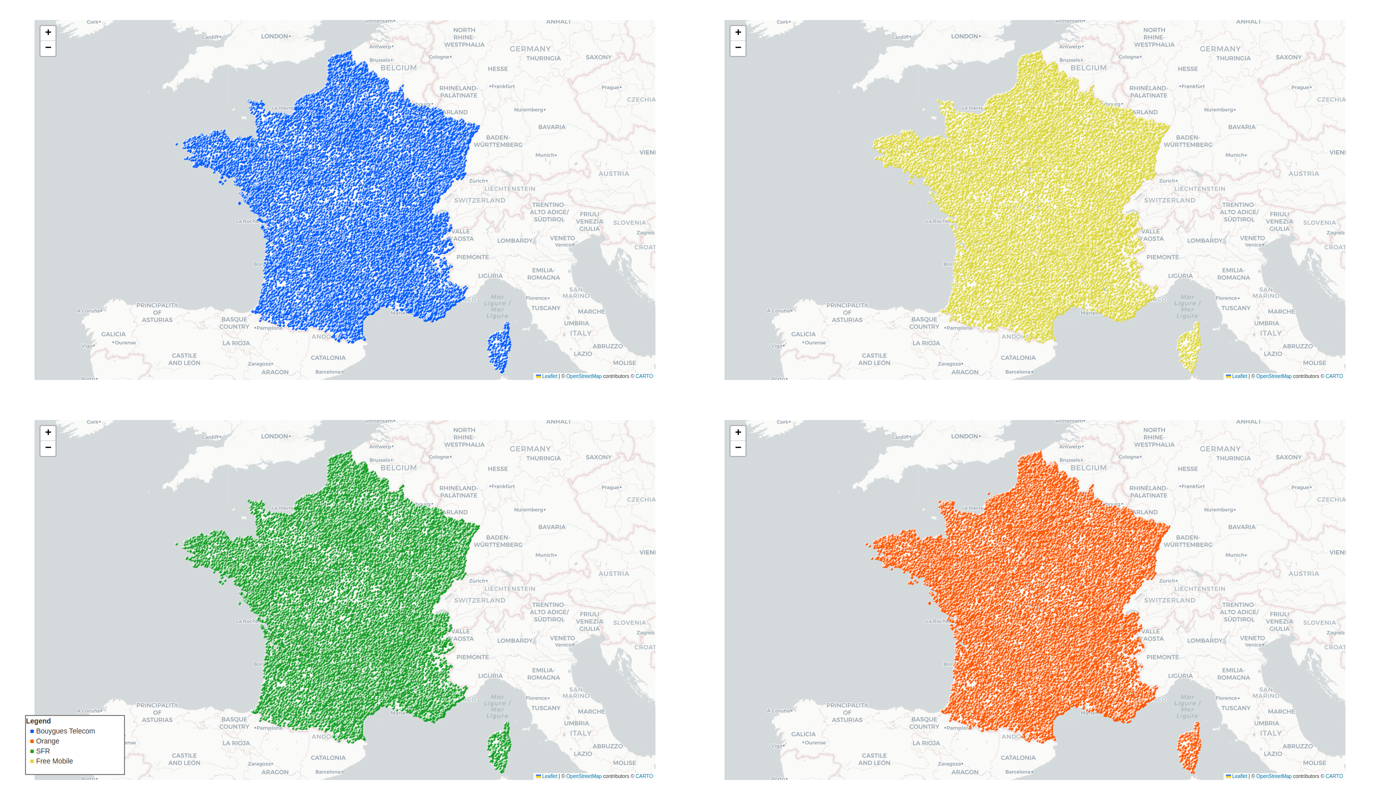
\includegraphics[width=0.9\paperheight]{images/cartes/providers-site_4g.png}
        \caption{\label{fig:sp-4g}Les stations 4G}
    \end{figure}
\end{frame}

\begin{frame}{Les stations 5G}
    \begin{figure}
        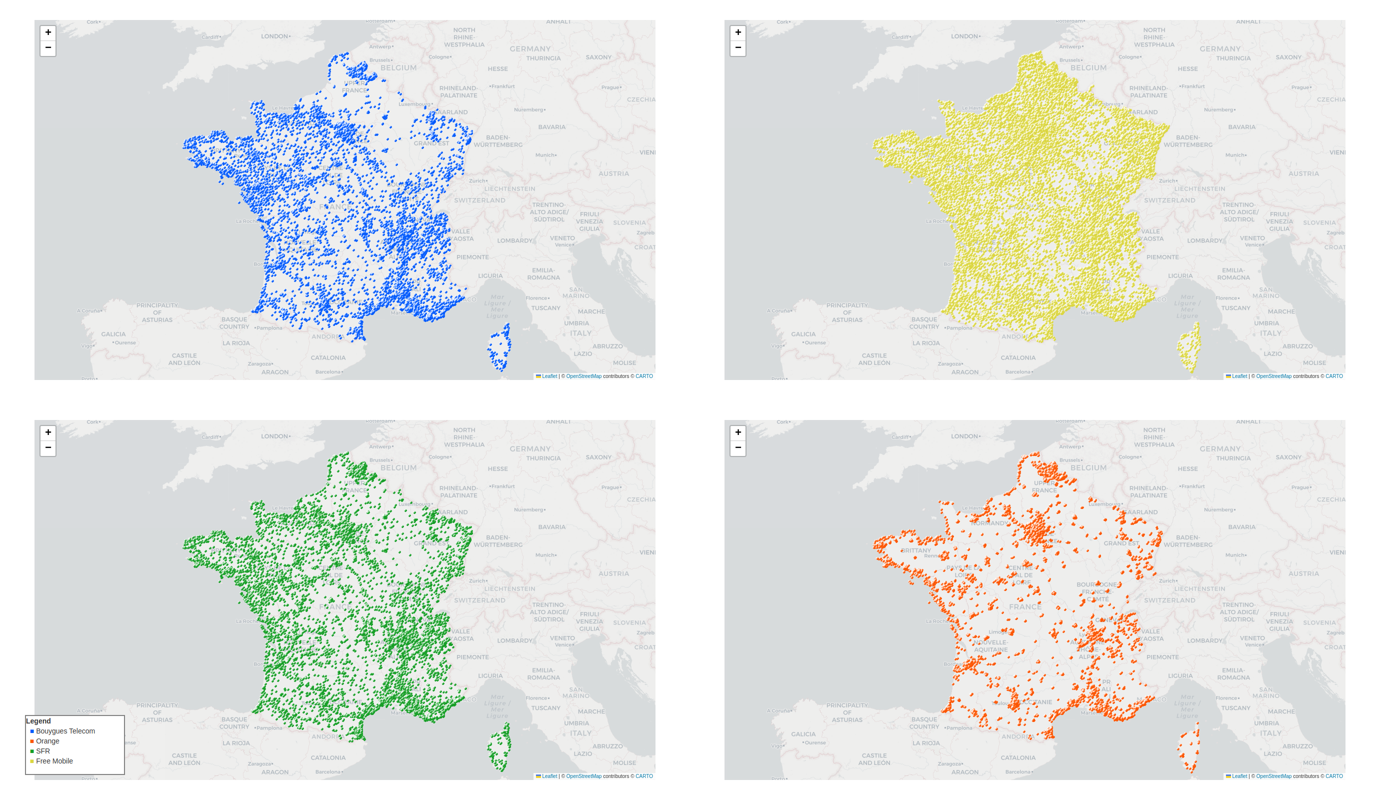
\includegraphics[width=0.9\paperheight]{images/cartes/providers-site_5g.png}
        \caption{\label{fig:sp-5g}Les stations 5G}
    \end{figure}
\end{frame}


\subsection{Evolution du nombre de stations de base au cours du temps}
\insertsubsectionframe

\begin{frame}{2023\_T4\_sites\_5G\_historique\_comptage}
    \begin{figure}
        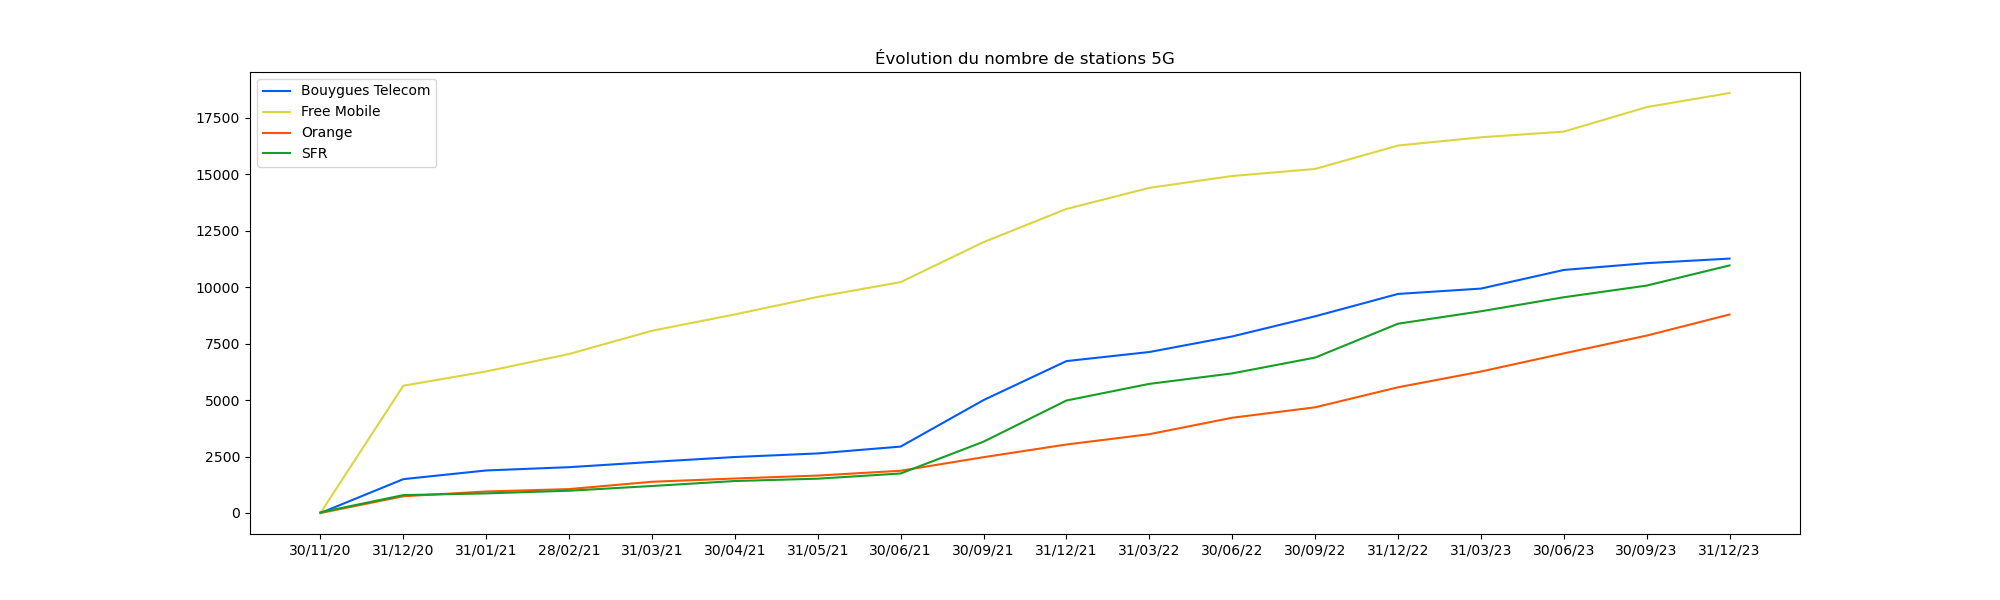
\includegraphics[height=0.5\paperheight]{images/5G-evolution.png}
        \caption{\label{fig:5G-ev}Evolution du nombre de stations 5G en France}
    \end{figure}
\end{frame}


\begin{frame}{}
    \begin{figure}
        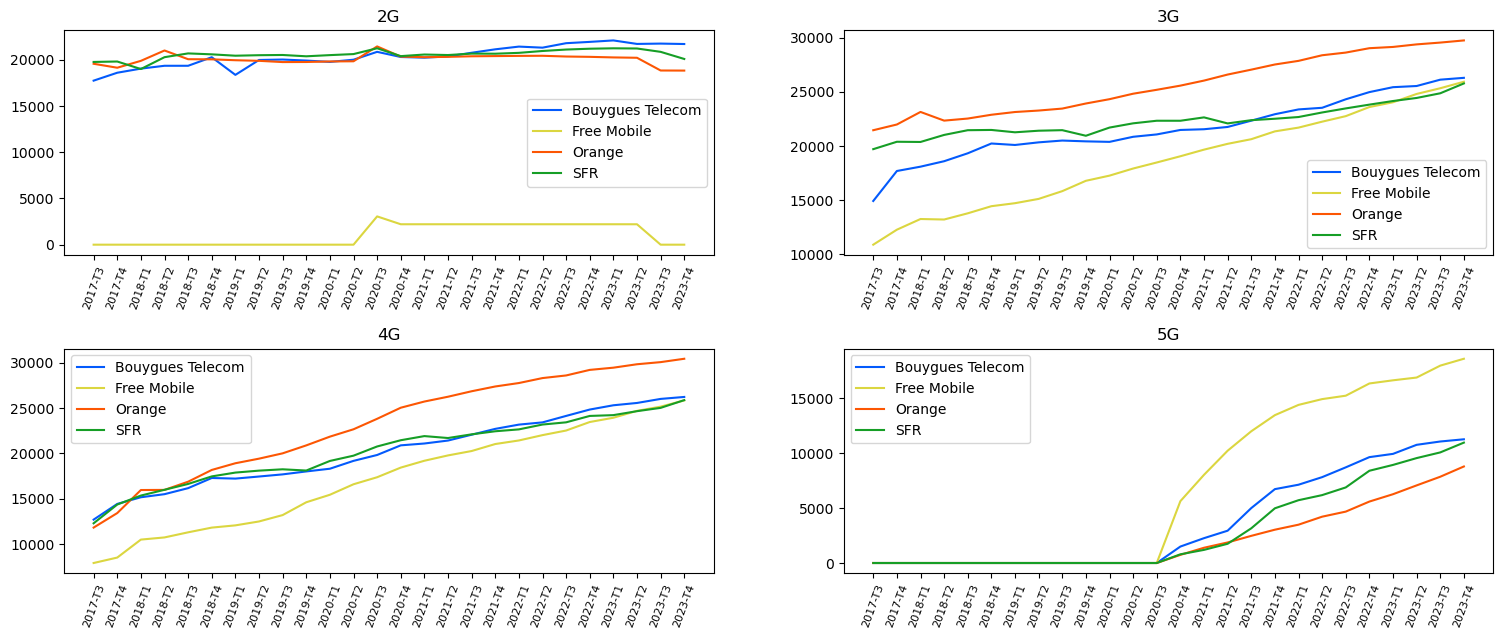
\includegraphics[height=0.8\paperheight]{images/technos-evolution.png}
        \caption{\label{fig:techno-ev}Compilation des jeux de données sites}
    \end{figure}
\end{frame}

\begin{frame}{Dispositif de couverture ciblée, éléments d'analyse}
    \begin{block}{infos générales}
        \begin{itemize}
            \item 4621 stations de bases potentielles;
            \item 26 attributs.
        \end{itemize}
    \end{block}

    \begin{block}{anomalies}
        \begin{itemize}
            \item 412 lignes de ce jeu de données ont les colonnes \textbf{x\_lambert\_93} ou \textbf{y\_lambert\_93} non renseigné;
            \item Plusieurs points sont placés en dehors de la France.
        \end{itemize}
    \end{block}
\end{frame}


\begin{frame}{Dispositif de couverture ciblée}
    \begin{figure}
        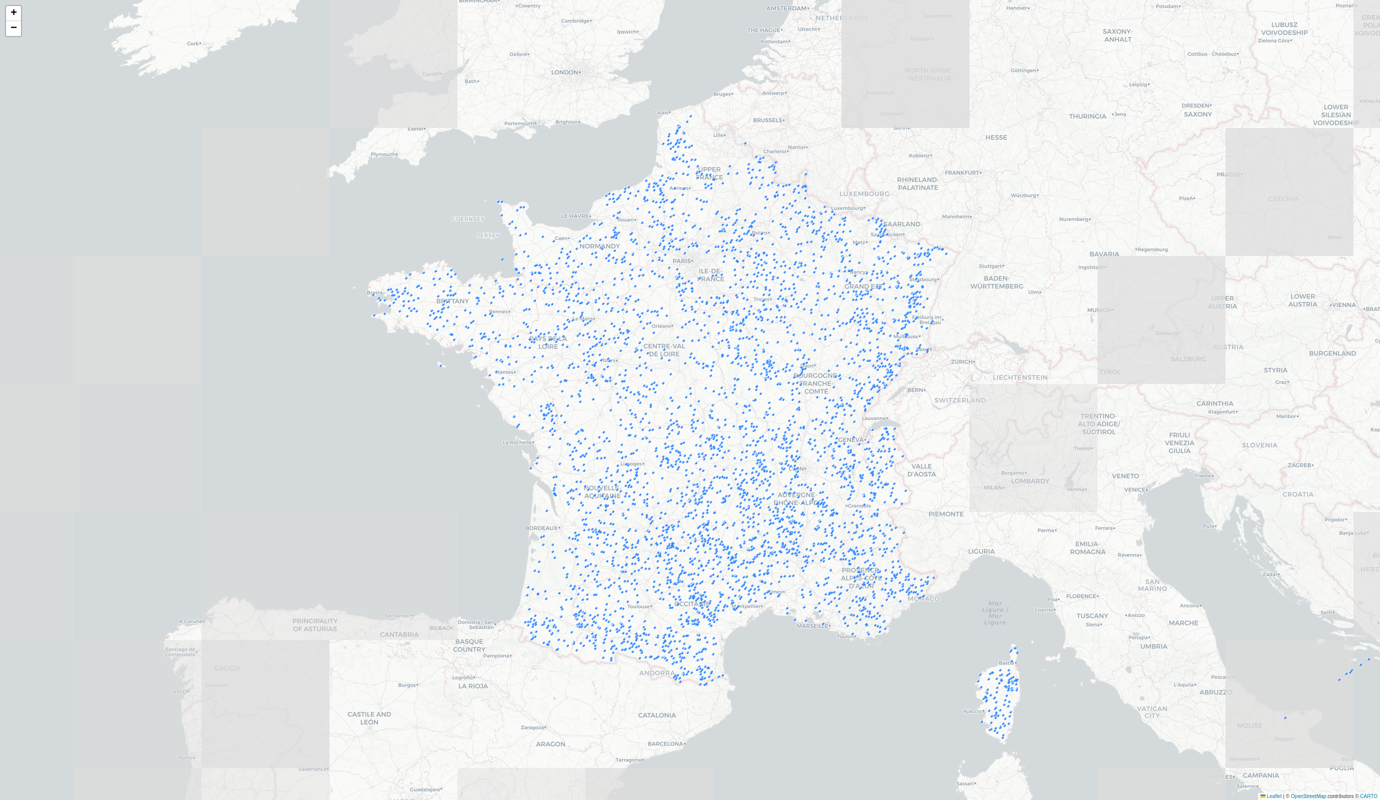
\includegraphics[height=.8\textheight]{images/couverture_ciblee.png}
    \end{figure}
\end{frame}

\smallframetitle

\section{Semaine du 21/05/24 au 28/05/24}
\insertsectionframe

\subsection{Statistiques stations de bases - départements}
\insertsubsectionframe

\begin{frame}{Méthodologie}
    On va utiliser une base de donnée complémentaire, reprise de celle trouvée l'année dernière.

    \begin{block}{Une nouvelle base de donnée\footnotemark}
        Cette base de donnée renseigne, par département, la \textbf{superficie} (en $\unit{km^2}$), la \textbf{population} et la \textbf{densité de population} au $\unit{km^2}$.
    \end{block}
    
    A partir de cette base, on va donc pouvoir extraire le nombre d'habitants par stations (normalisé par la taille du département) et la densité de station par département.

    \begin{block}{Calcul du nombre d'habitants par stations normalisé}
        Soit $\lambda$ le nombre d'habitants par stations, par $\unit{km^2}$. Tout d'abord, on se donne $\gamma$, le rapport entre le nombre d'habitant et la surface du département, qui est donné par la densité de population.
        Ensuite, on calcule notre résultat comme suit :$$\lambda = \gamma\times\frac{1}{\text{nombre de stations du département}}$$
    \end{block}

    \footnotetext{\url{https://france.ousuisje.com/departements/classement/superficie.php}}
\end{frame}

\begin{frame}{Nombre d'habitants par stations non normalisé}
    C'est le même calcul que précédemment, sauf qu'à la place de $\gamma$, on utilise simplement la population du département.
    \begin{figure}
        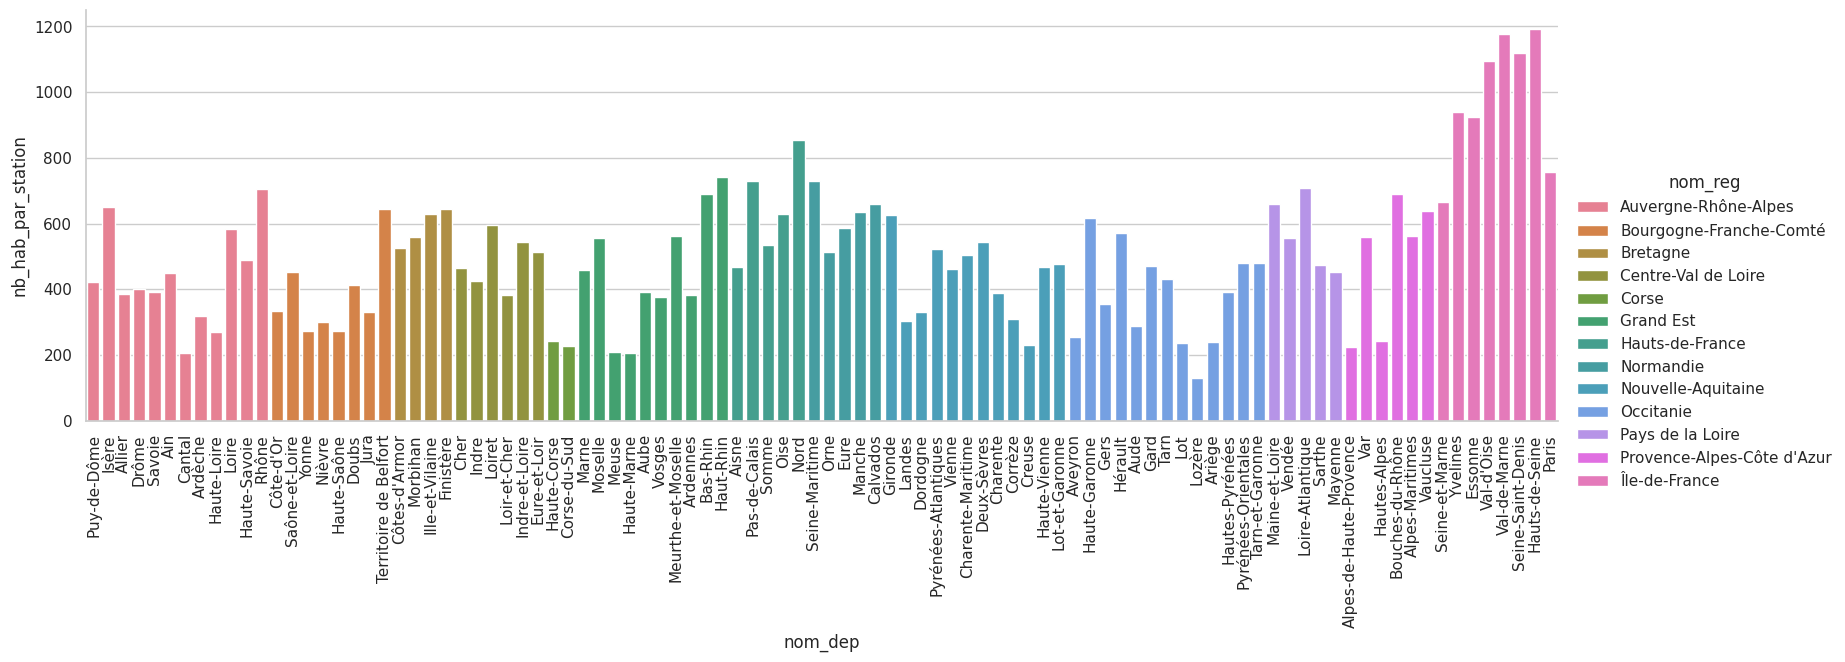
\includegraphics[width=0.9\paperwidth]{images/barplots/nb_hab_par_station_par_dep.png}
        \caption{\label{fig:nb_hap_par_stat_par_dep}Répartition du nombre d'habitants par station, en fonction du département}
    \end{figure}
\end{frame}

\begin{frame}{Nombre d'habitants par stations normalisé (1/2)}
    \begin{figure}
        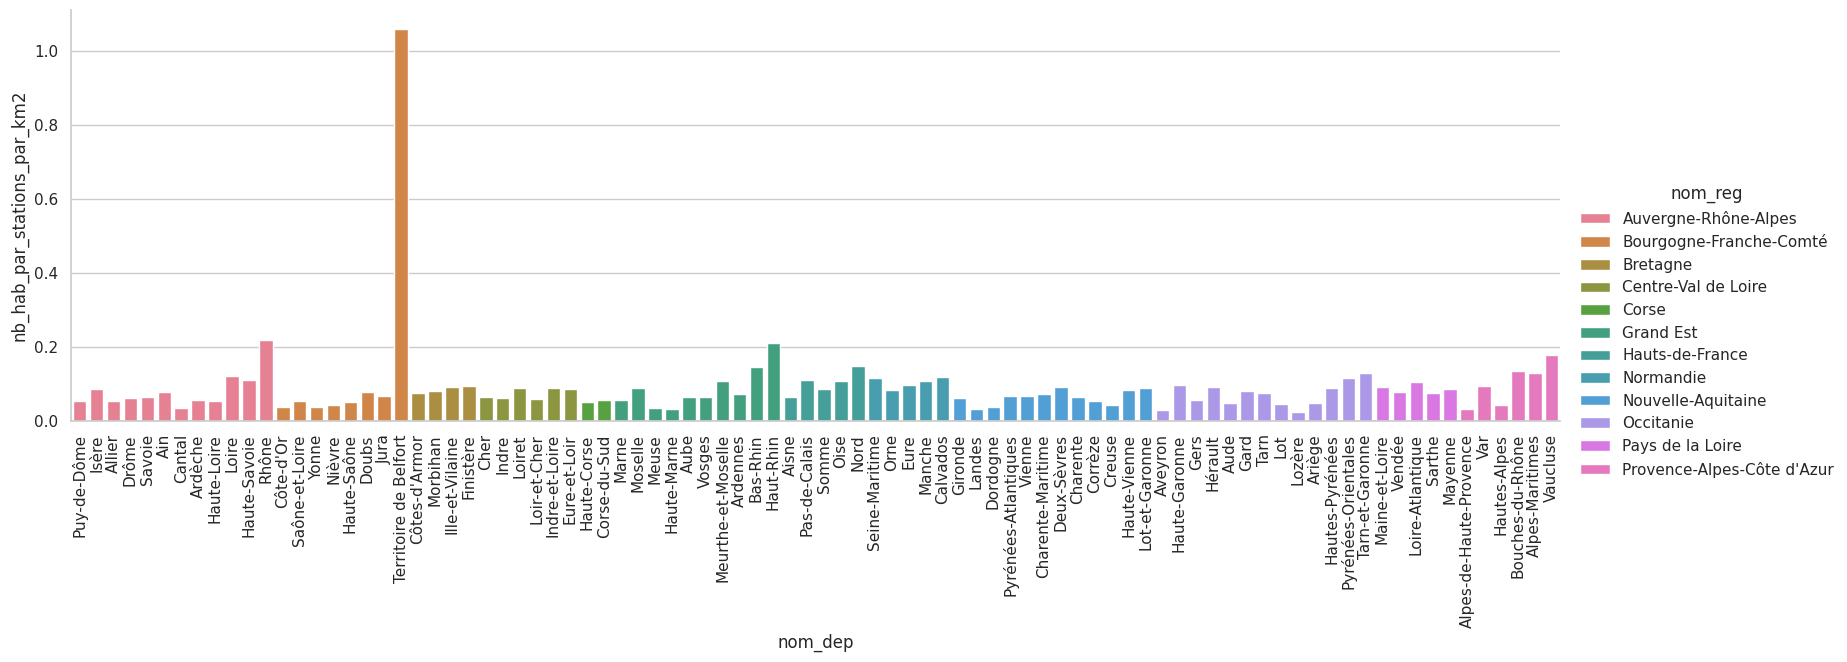
\includegraphics[width=0.9\paperwidth]{images/barplots/nb_hab_par_stations_par_km2_sansIDF.png}
        \caption{\label{fig:nb_hap_par_stat_par_dep_norm_ssIDF}Répartition du nombre d'habitants par station, en fonction du département (normalisé), sans l'Île-de-France}
    \end{figure}
\end{frame}

\begin{frame}{Nombre d'habitants par stations normalisé (2/2)}
    \begin{figure}
        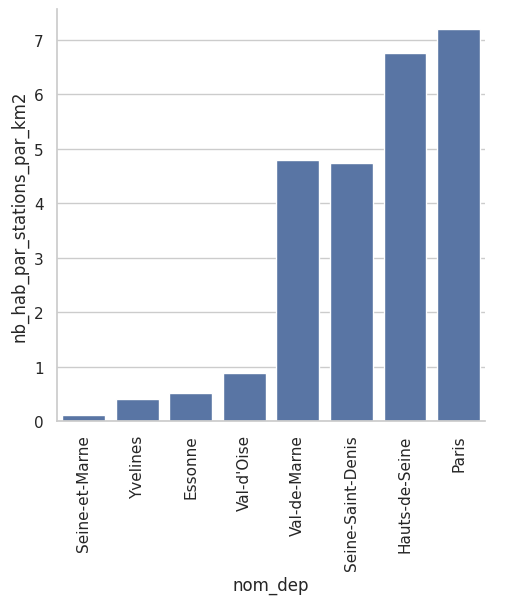
\includegraphics[height=0.55\paperheight]{images/barplots/nb_hab_par_stations_par_km2_IDF.png}
        \caption{\label{fig:nb_hap_par_stat_par_dep_norm_IDF}Répartition du nombre d'habitants par station, en fonction du département (normalisé), sur l'Île-de-France}
    \end{figure}
\end{frame}

\begin{frame}{Densité de stations (1/2)}
    \begin{figure}
        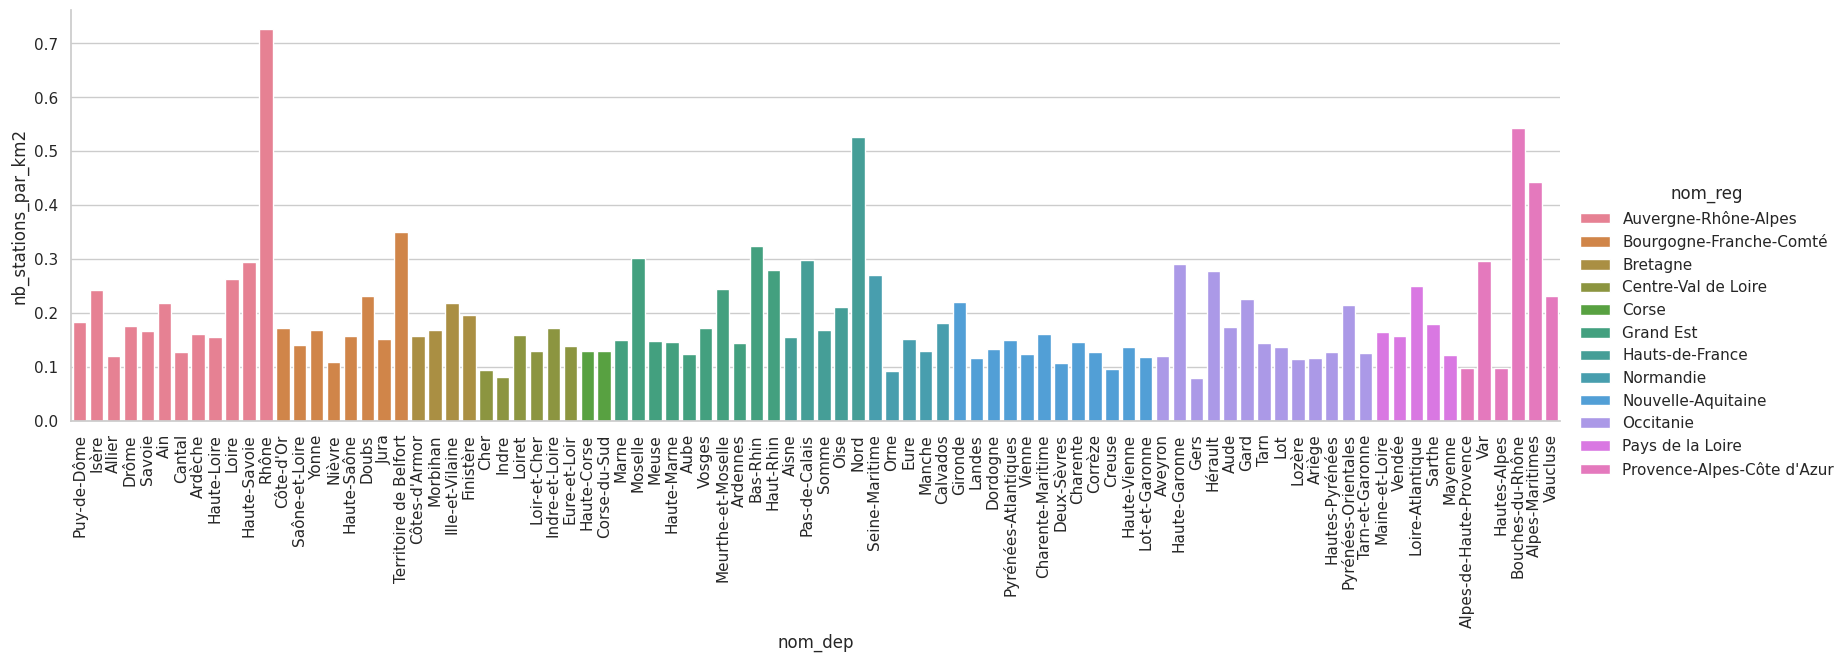
\includegraphics[width=0.9\paperwidth]{images/barplots/densite_station_par_dep_sansIDF.png}
        \caption{\label{fig:densite_stat_ssIDF}Nombre de stations de base au $\unit{km^2}$, sans l'Île-de-France}
    \end{figure}
\end{frame}

\begin{frame}{Densité de stations (2/2)}
    \begin{figure}
        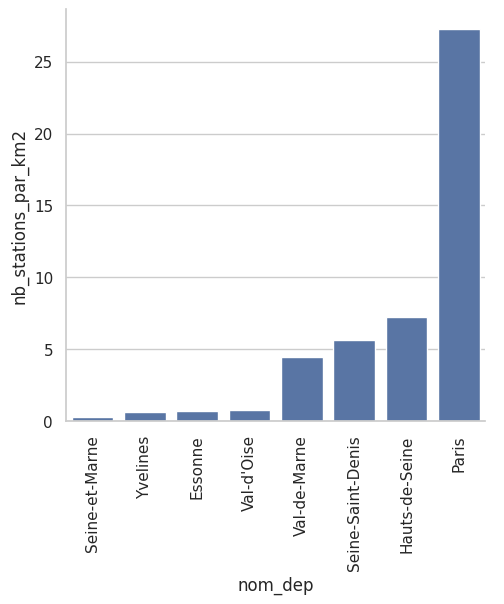
\includegraphics[height=0.55\paperheight]{images/barplots/densite_station_par_dep_IDF.png}
        \caption{\label{fig:densite_stat_IDF}Nombre de stations de base au $\unit{km^2}$, sur l'Île-de-France}
    \end{figure}
\end{frame}

\begin{frame}{Fréquences d'émission des stations 5G}
    \begin{figure}
        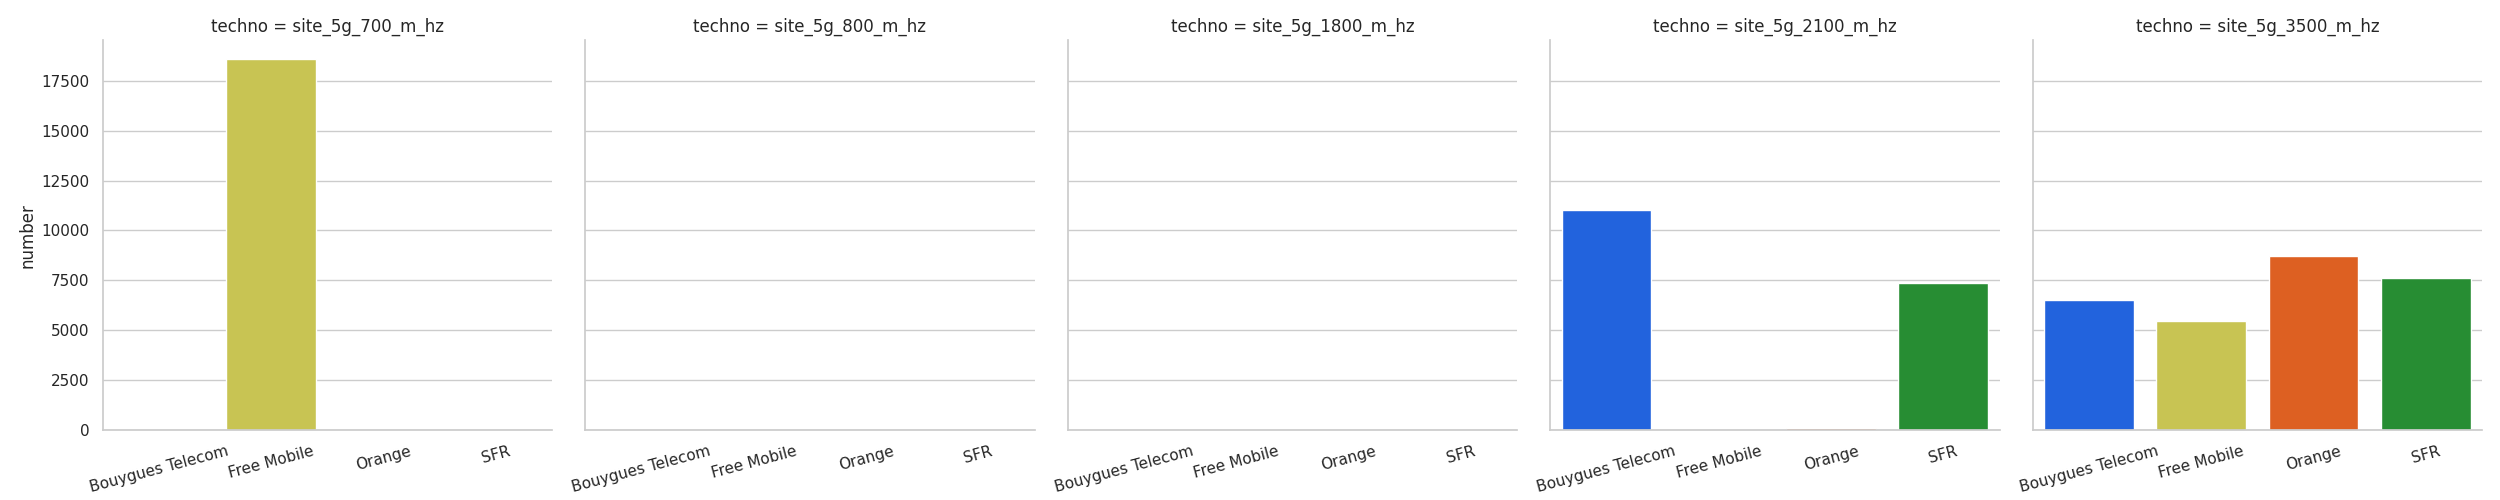
\includegraphics[width=0.9\paperwidth]{images/barplots/5G_freq.png}
        \caption{\label{fig:5g_freq}Répartition des fréquences d'émission des stations 5G, en fonction des opérateurs}
    \end{figure}
\end{frame}

\subsection{Détection de voisins - méthode PAQUIRY}
\insertsubsectionframe

\begin{frame}{Principe général}
    La recherche de voisins va s'articuler atour de deux axes :
    \begin{block}{Triangulation de Delaunay}
        On crée un graphe de voisinage grâce à la triangulation de Delaunay. Ceci nous donne donc, pour chaque station de base, une liste de voisins potentiels.
        Il faut ensuite vérifier que ce sont bien des voisins réels.
    \end{block}
    \begin{block}{Critères de sélection}
        Pour être sûr qu'un voisin est un voisin réel on applique trois critères, dans l'ordre suivant :
        \begin{enumerate}
            \item la distance maximale ;
            \item le plus proche voisin dans un cadrant ;
            \item l'angle minimum entre deux voisins.
        \end{enumerate}
    \end{block}
    Cette méthode a été élaborée par Delphine PAQUIRY l'été dernier.
\end{frame}

\begin{frame}{Critère de distance}
    \begin{columns}
        \begin{column}{0.4\paperwidth}
            \begin{block}{Principe}
                Ici, on élimine tous les voisins qui sont distants de plus de $\unit[15]{km}$.
            \end{block}
            \begin{block}{Intérêt du critère}
                Il est logique de penser que deux stations trop éloignées géographiquement ne sont pas voisines.
            \end{block}
        \end{column}
        \begin{column}{0.55\paperwidth}
            \begin{figure}
                \boxed{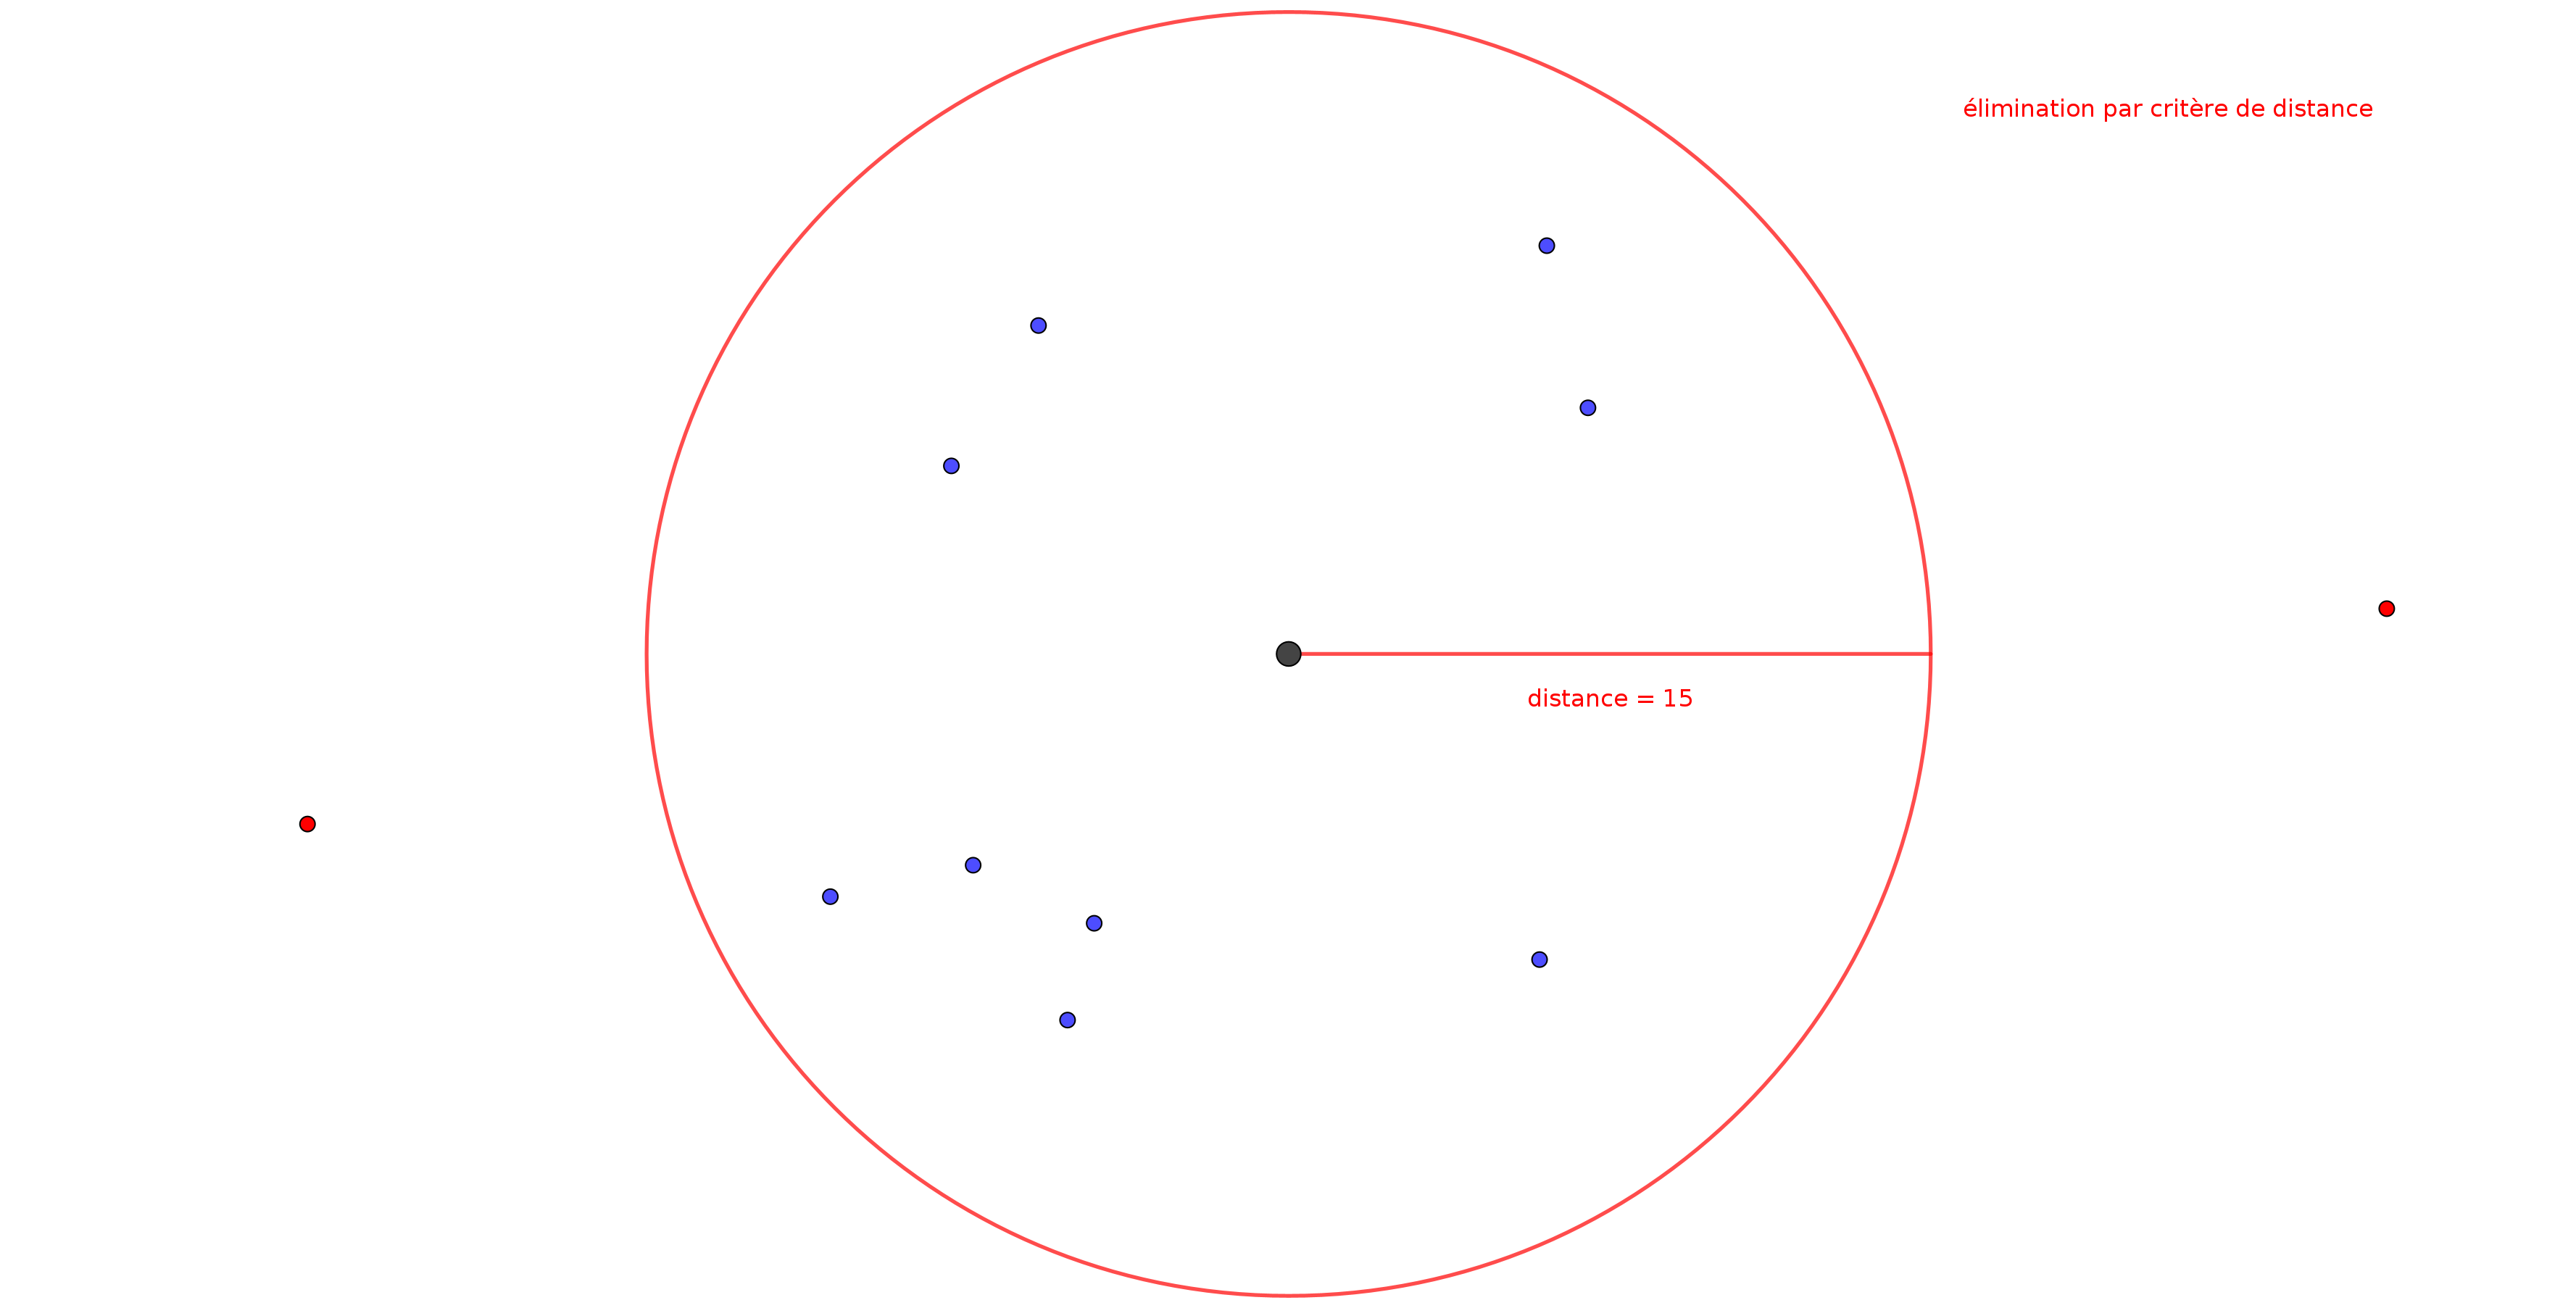
\includegraphics[width=0.5\paperwidth]{images/criteria_illustrations/distance.png}}
                \caption{\label{fig:distance_crit}Illustration du critère de distance}
            \end{figure}
        \end{column}
    \end{columns}
\end{frame}

\begin{frame}{Critère des cadrants}
    \begin{columns}
        \begin{column}{0.4\paperwidth}
            \begin{block}{Principe}
                Ici, on ne garde que le plus proche voisin dans un cadrant. On a choisi 6 cadrants car c'est le chiffre qui nous donne les meilleurs résultats.
            \end{block}
            \begin{block}{Intérêt du critère}
                On évite les effets de cluster.
            \end{block}
        \end{column}
        \begin{column}{0.55\paperwidth}
            \begin{figure}
                \boxed{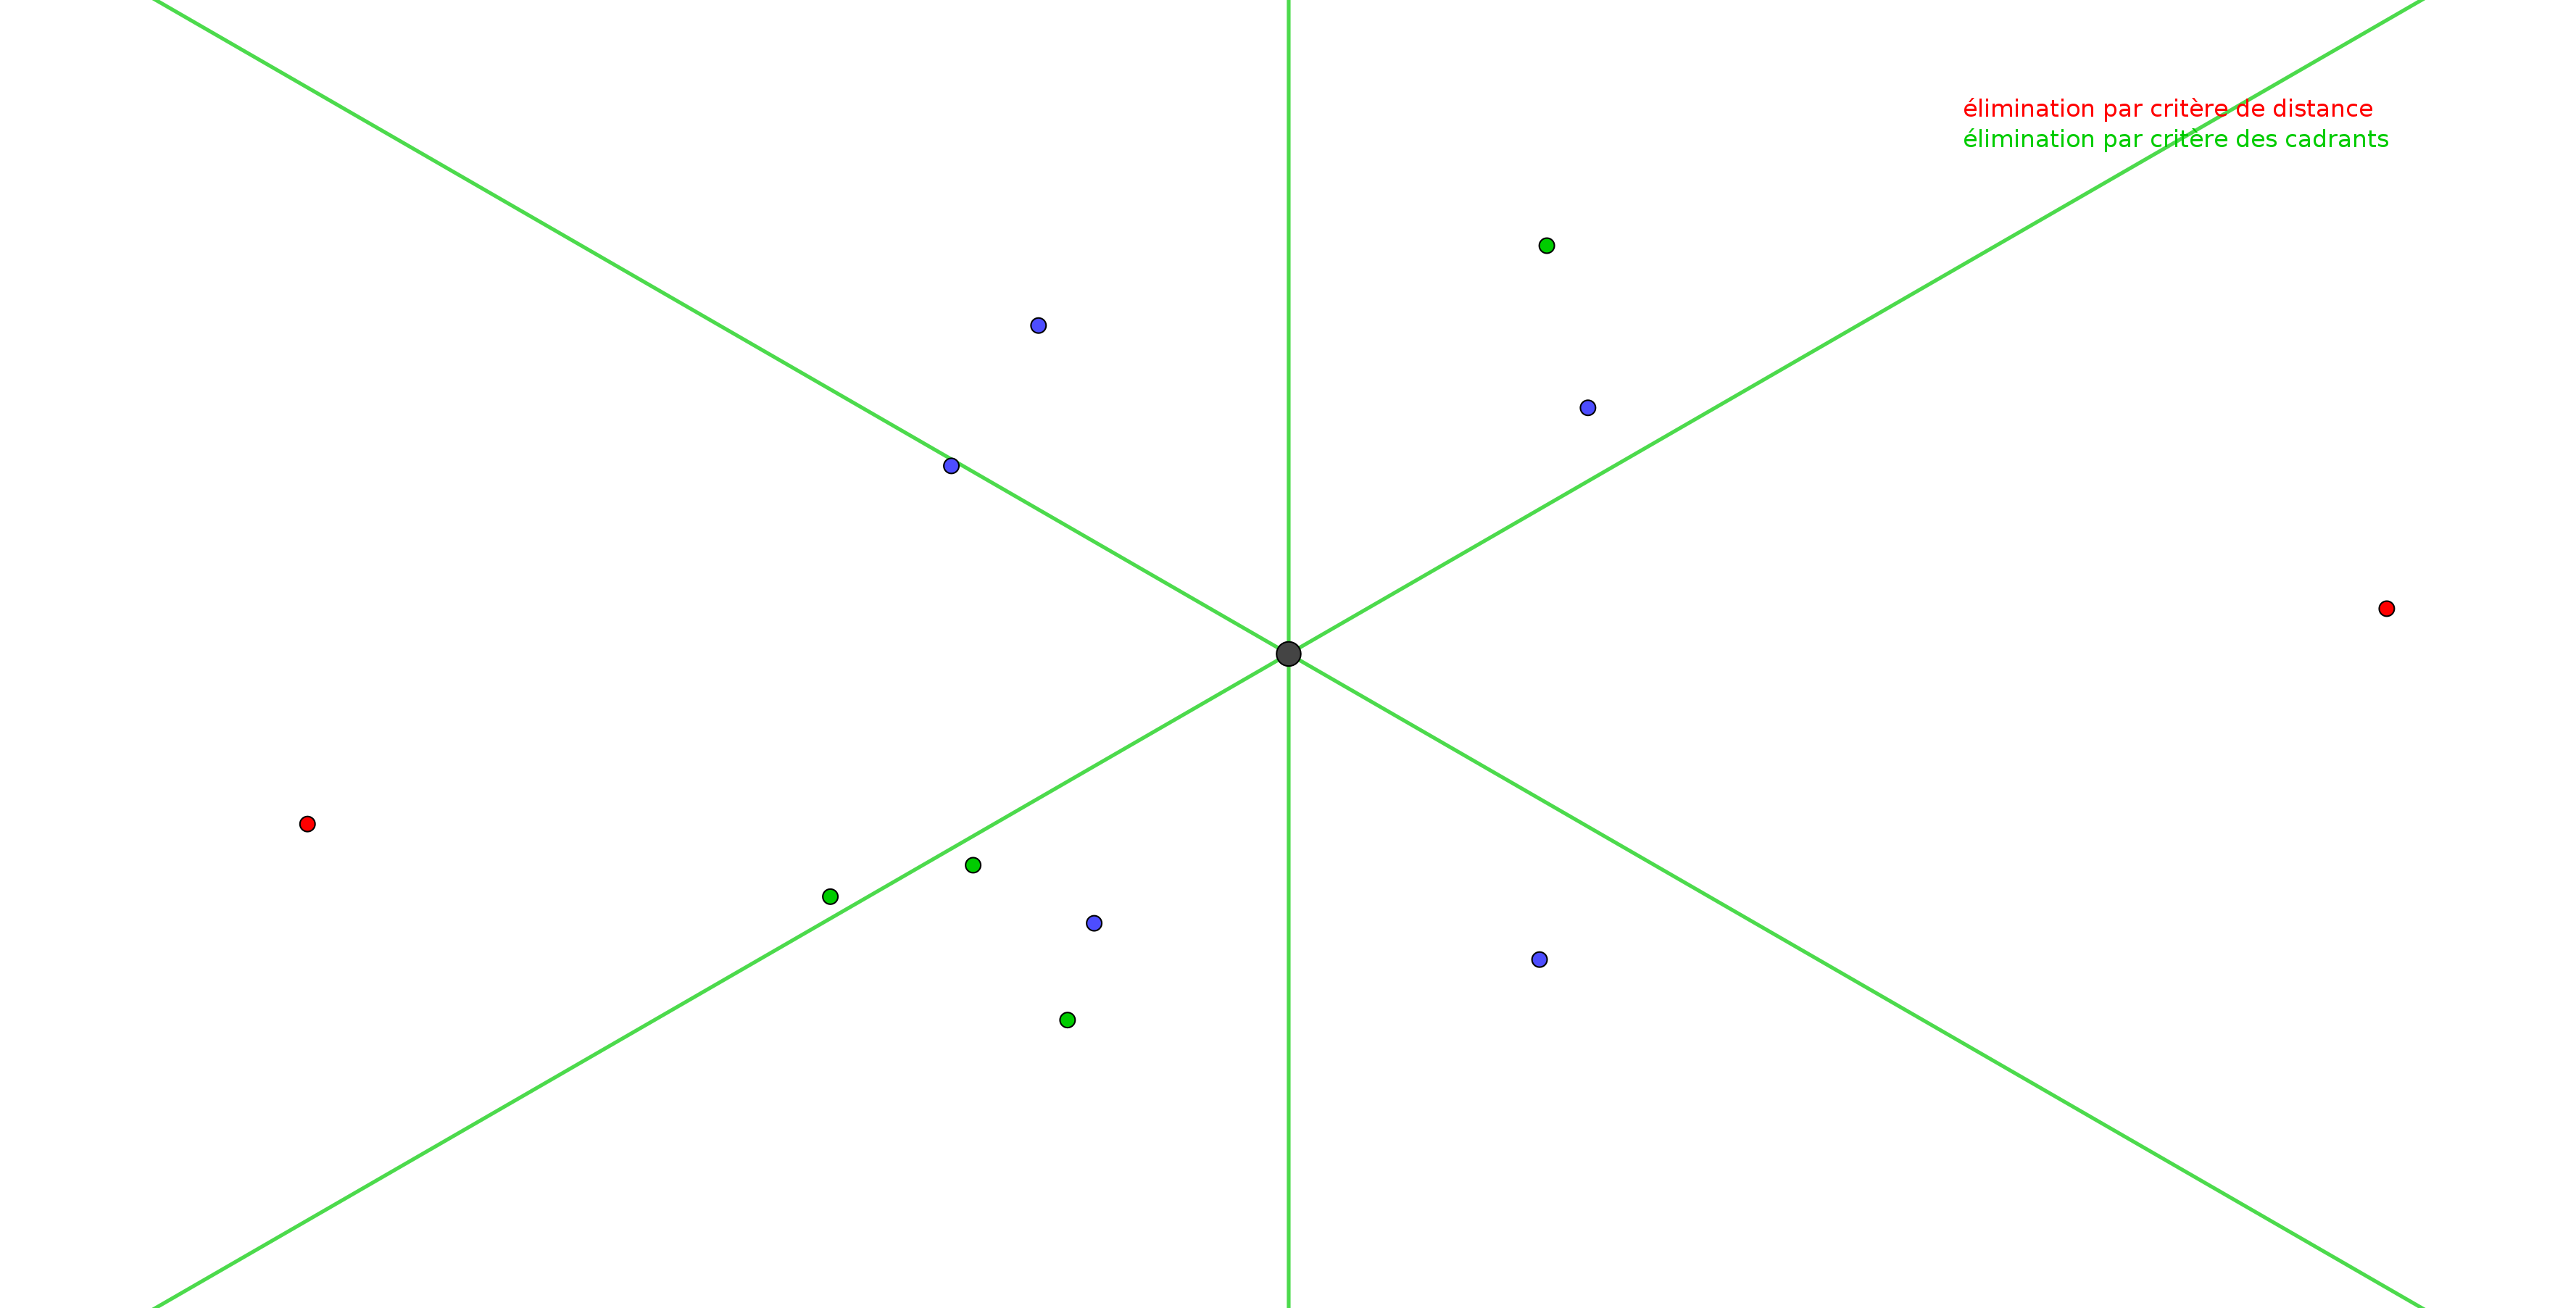
\includegraphics[width=0.5\paperwidth]{images/criteria_illustrations/cadrants.png}}
                \caption{\label{fig:cadrants_crit}Illustration du critère des cadrants}
            \end{figure}
        \end{column}
    \end{columns}
\end{frame}

\begin{frame}{Critère de l'angle}
    \begin{columns}
        \begin{column}{0.4\paperwidth}
            \begin{block}{Principe}
                Ici, si deux voisins sont séparés d'un angle inférieur à $30^{\circ}$, on ne garde que le plus proche. Cette valeur d'angle est arbitraire et pourrait être variable en fonction de l'urbanité de la station.
            \end{block}
            \begin{block}{Intérêt du critère}
                Si deux stations sont trop proches angulairement parlant, la plus proche fait écran par rapport à la plus éloignée.
            \end{block}
        \end{column}
        \begin{column}{0.55\paperwidth}
            \begin{figure}
                \boxed{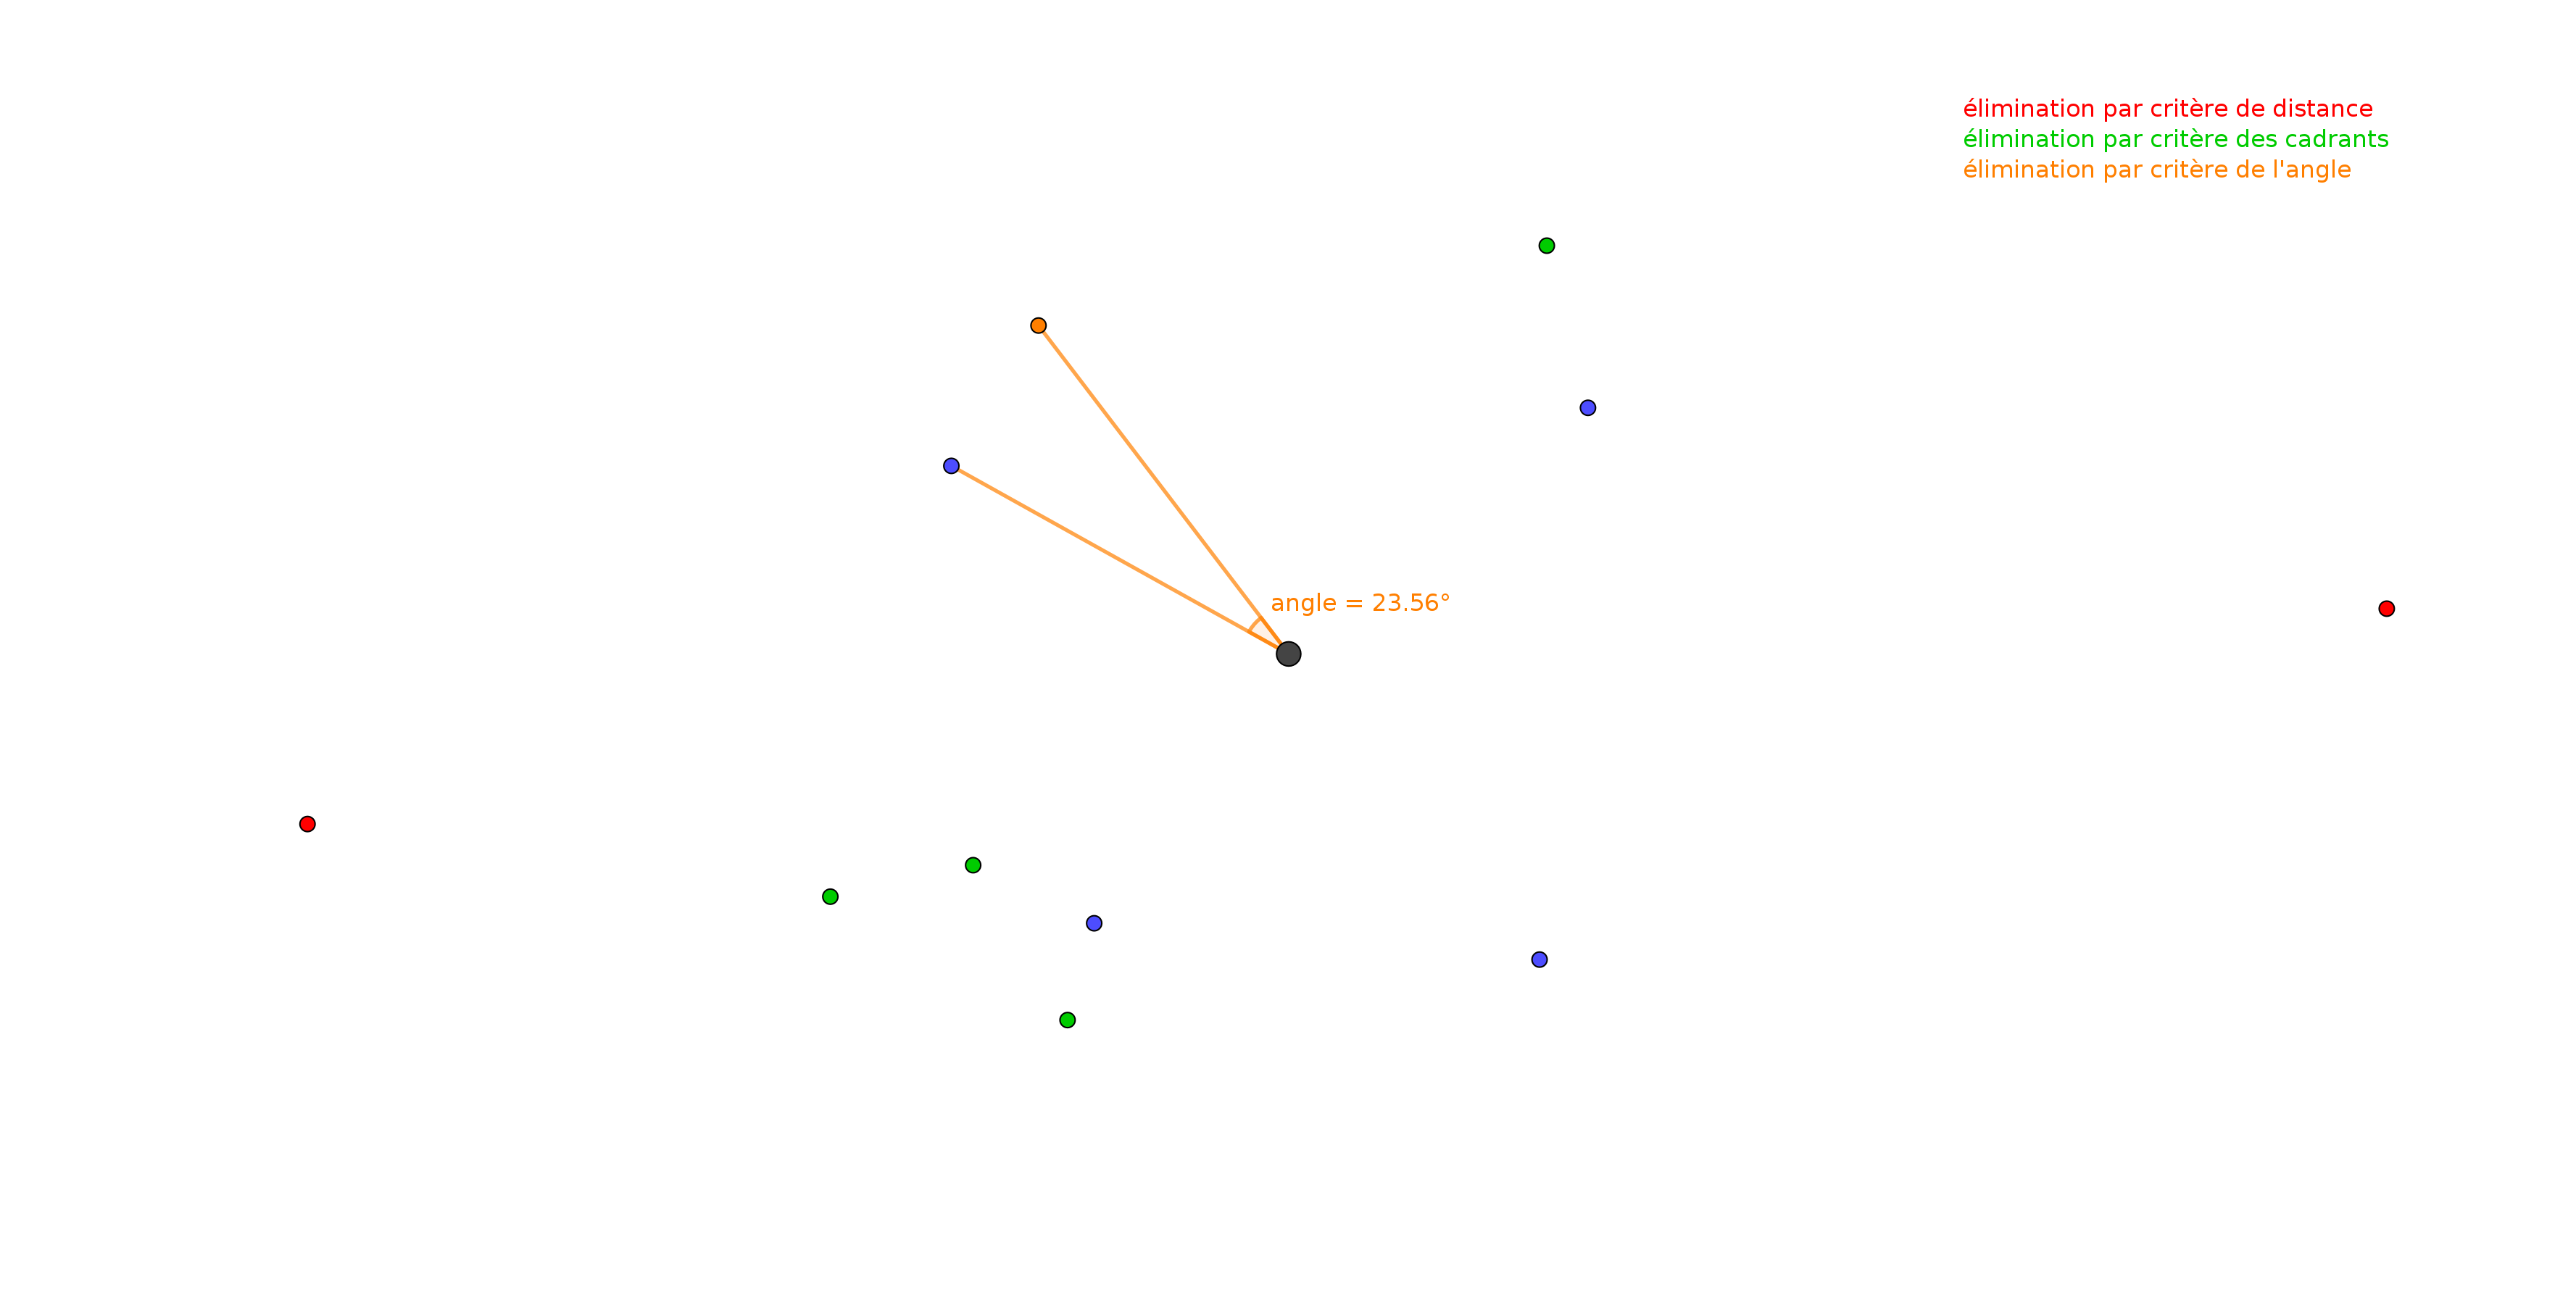
\includegraphics[width=0.5\paperwidth]{images/criteria_illustrations/angle.png}}
                \caption{\label{fig:angle_crit}Illustration du critère de l'angle}
            \end{figure}
        \end{column}
    \end{columns}
\end{frame}

\begin{frame}{Voisins réels}
    Voici donc ce que l'on obtient à la fin, un graphe de voisinage :
    \begin{figure}
        \boxed{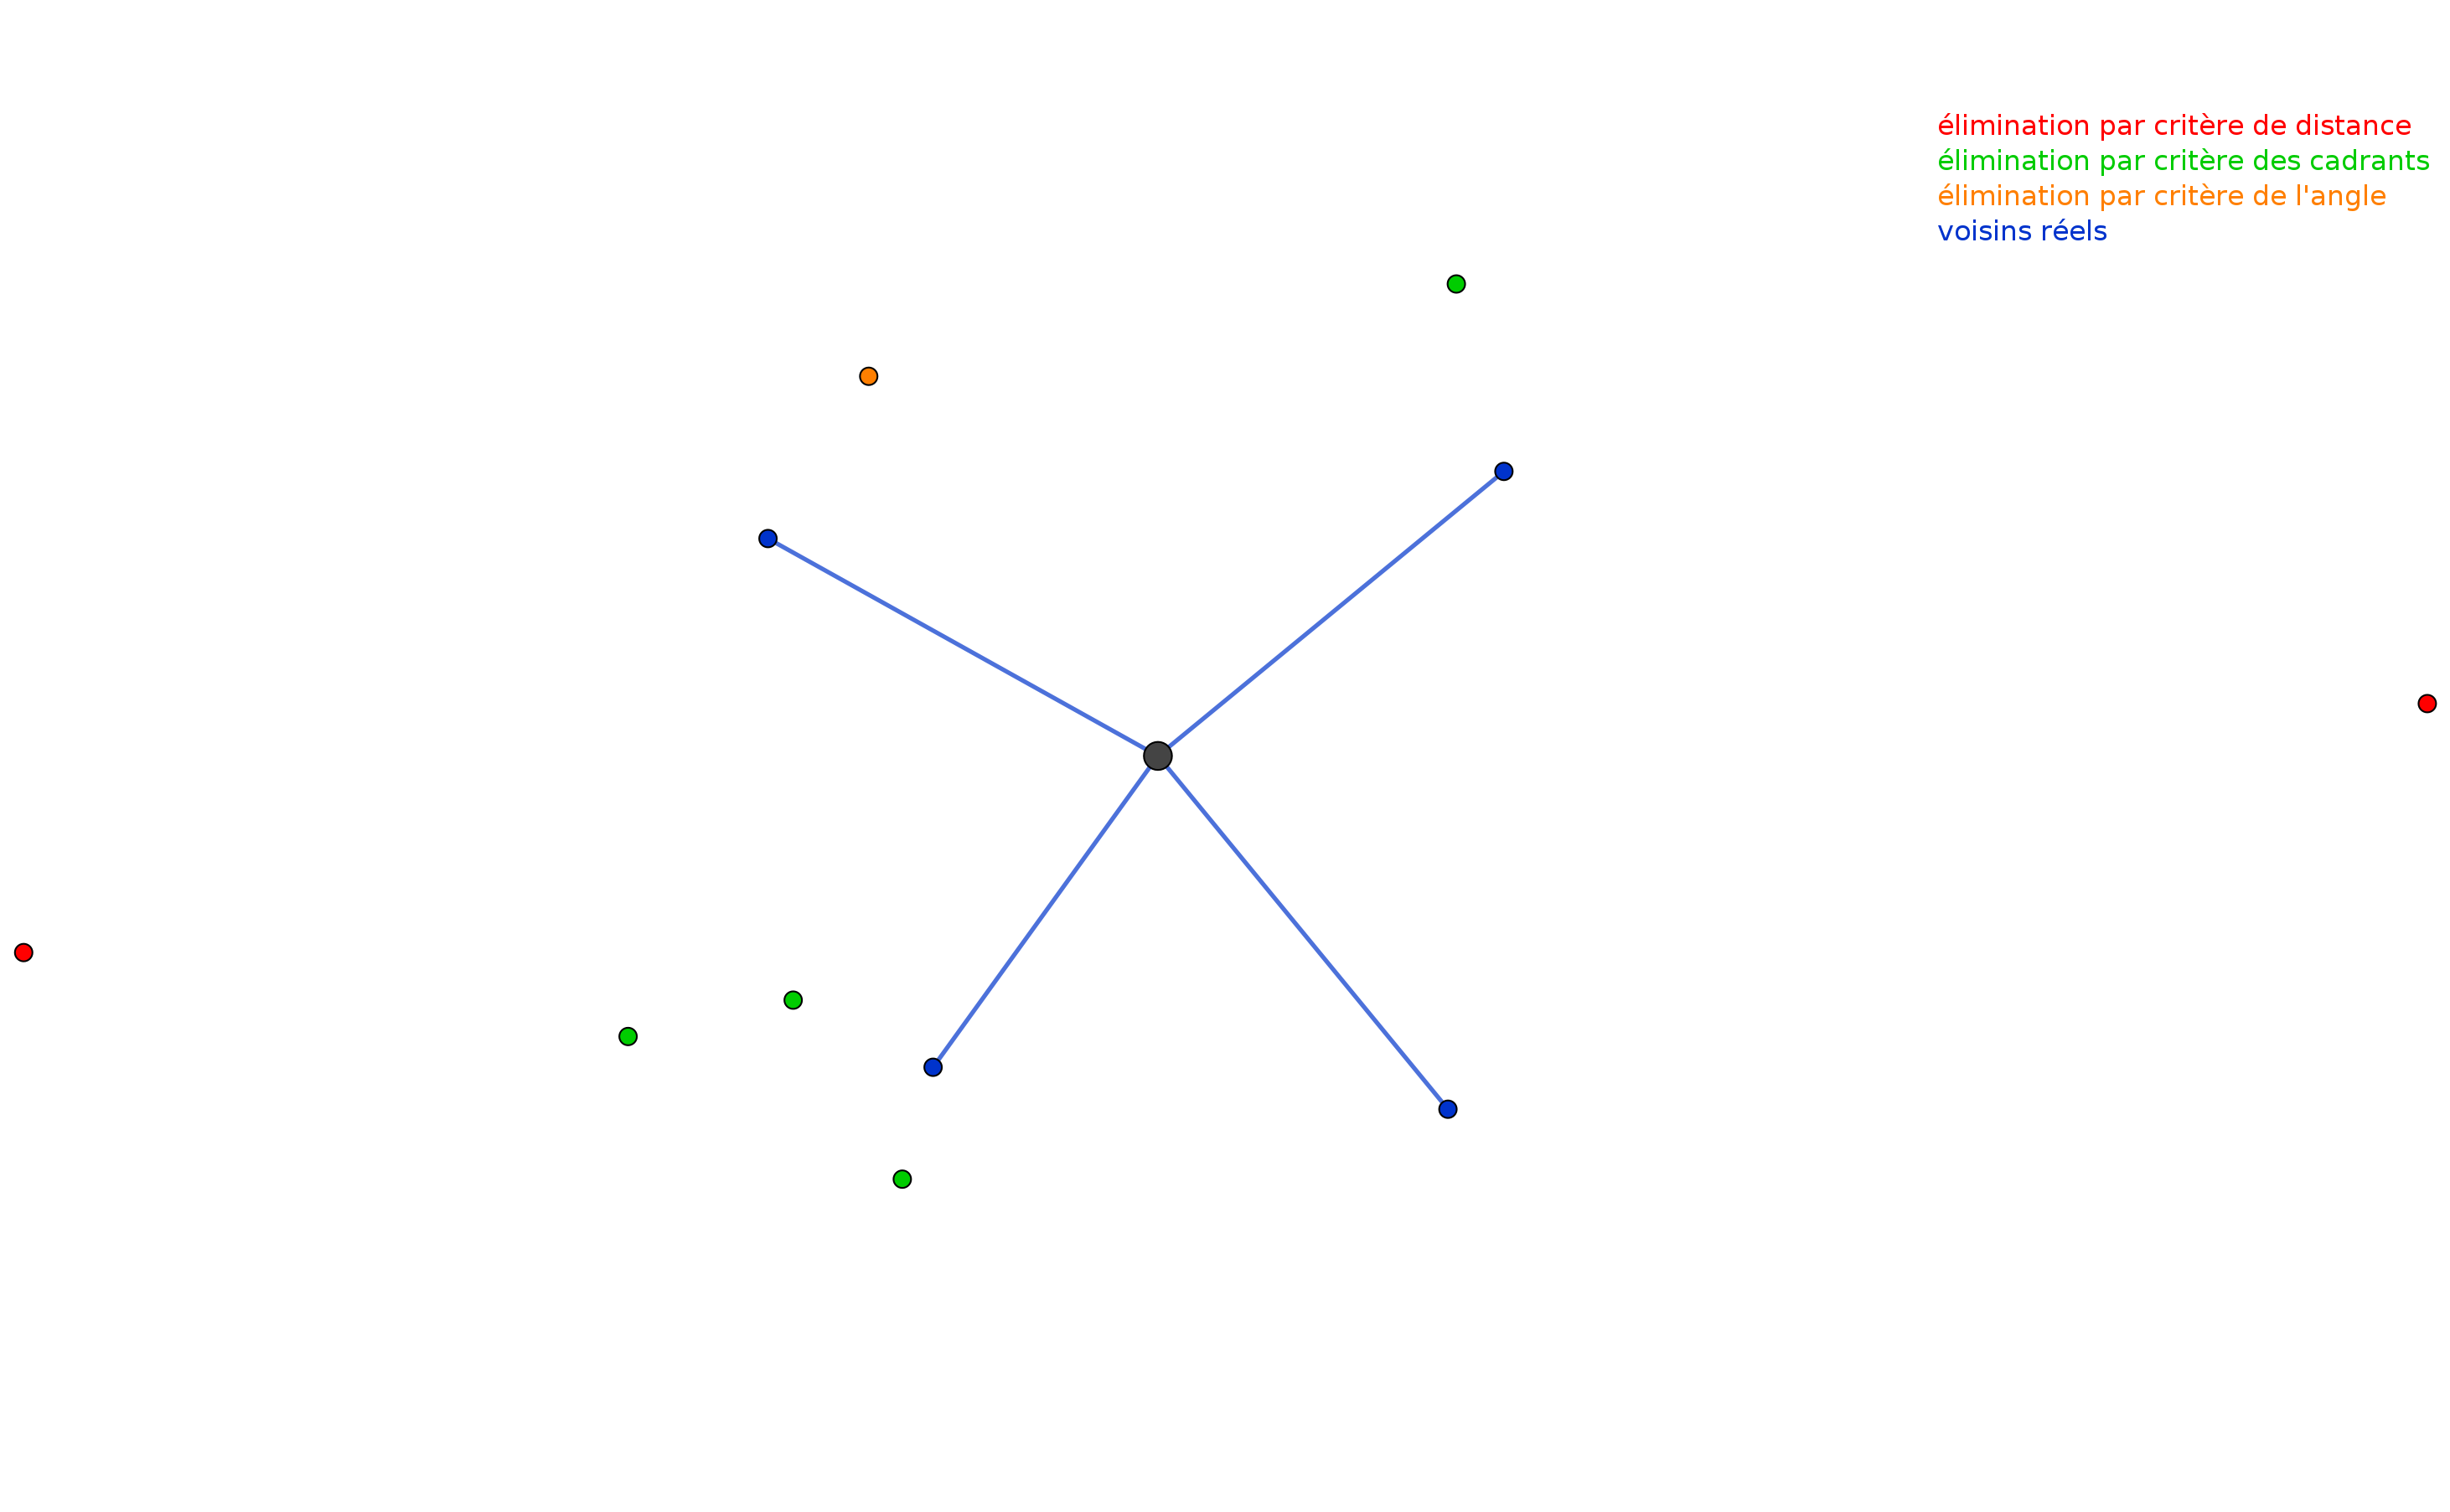
\includegraphics[height=0.55\paperheight]{images/criteria_illustrations/final.png}}
        \caption{\label{fig:result_crit}Résultat final - voisins réels}
    \end{figure}
\end{frame}

\subsection{Détection automatique des villes}
\insertsubsectionframe

\begin{frame}{DBScan}
    \begin{block}{Principe}
        \begin{itemize}
            \item Méthode de référence de la classification à densité (détection de clusters en se basant sur la concentration de points);
            \item Se base sur deux paramètres : $\varepsilon$ et $n_{min}$ qui caractérisent respectivement la distance maximale pour que deux points soient considérés \og proches \fg{} et la quantité minimale de points proches pour qu'un cluster soit créé.
        \end{itemize}
    \end{block}

    \begin{block}{Inconvénients}
        \begin{itemize}
            \item Le choix du paramètre $\varepsilon$ est hasardeux;
            \item Ne se comporte pas bien avec des jeux de données avec des clusters de densité variable (certains clusters avec des points plus rapprochés que d'autres);
            \item Réagit mal au bruit;
            \item Est binaire : un point appartient ou n'appartient pas à un cluster, pas d'entre deux.
        \end{itemize}
    \end{block}
\end{frame}

\begin{frame}{Fonctionnement DBScan (1/2)}

    \begin{columns}
        \begin{column}{0.40\textwidth}
            \begin{block}{Etape 0 : Initialisation}
                Soient n points de $\mathbb{R}^p$, $\epsilon \in \mathbb{R}$ et $n_{min} \in \mathbb{N}$.

                Ici, on prend $n_{min}=3$ et $\epsilon=2$
            \end{block}

            \begin{block}{Etape 1 - Les voisins}
                Pour chaque point, on cherche tous les points à une distance inférieure à $\epsilon$ (dont lui même). On les appelera les voisins.
            \end{block}
        \end{column}

        \begin{column}{0.60\textwidth}
            \begin{figure}
                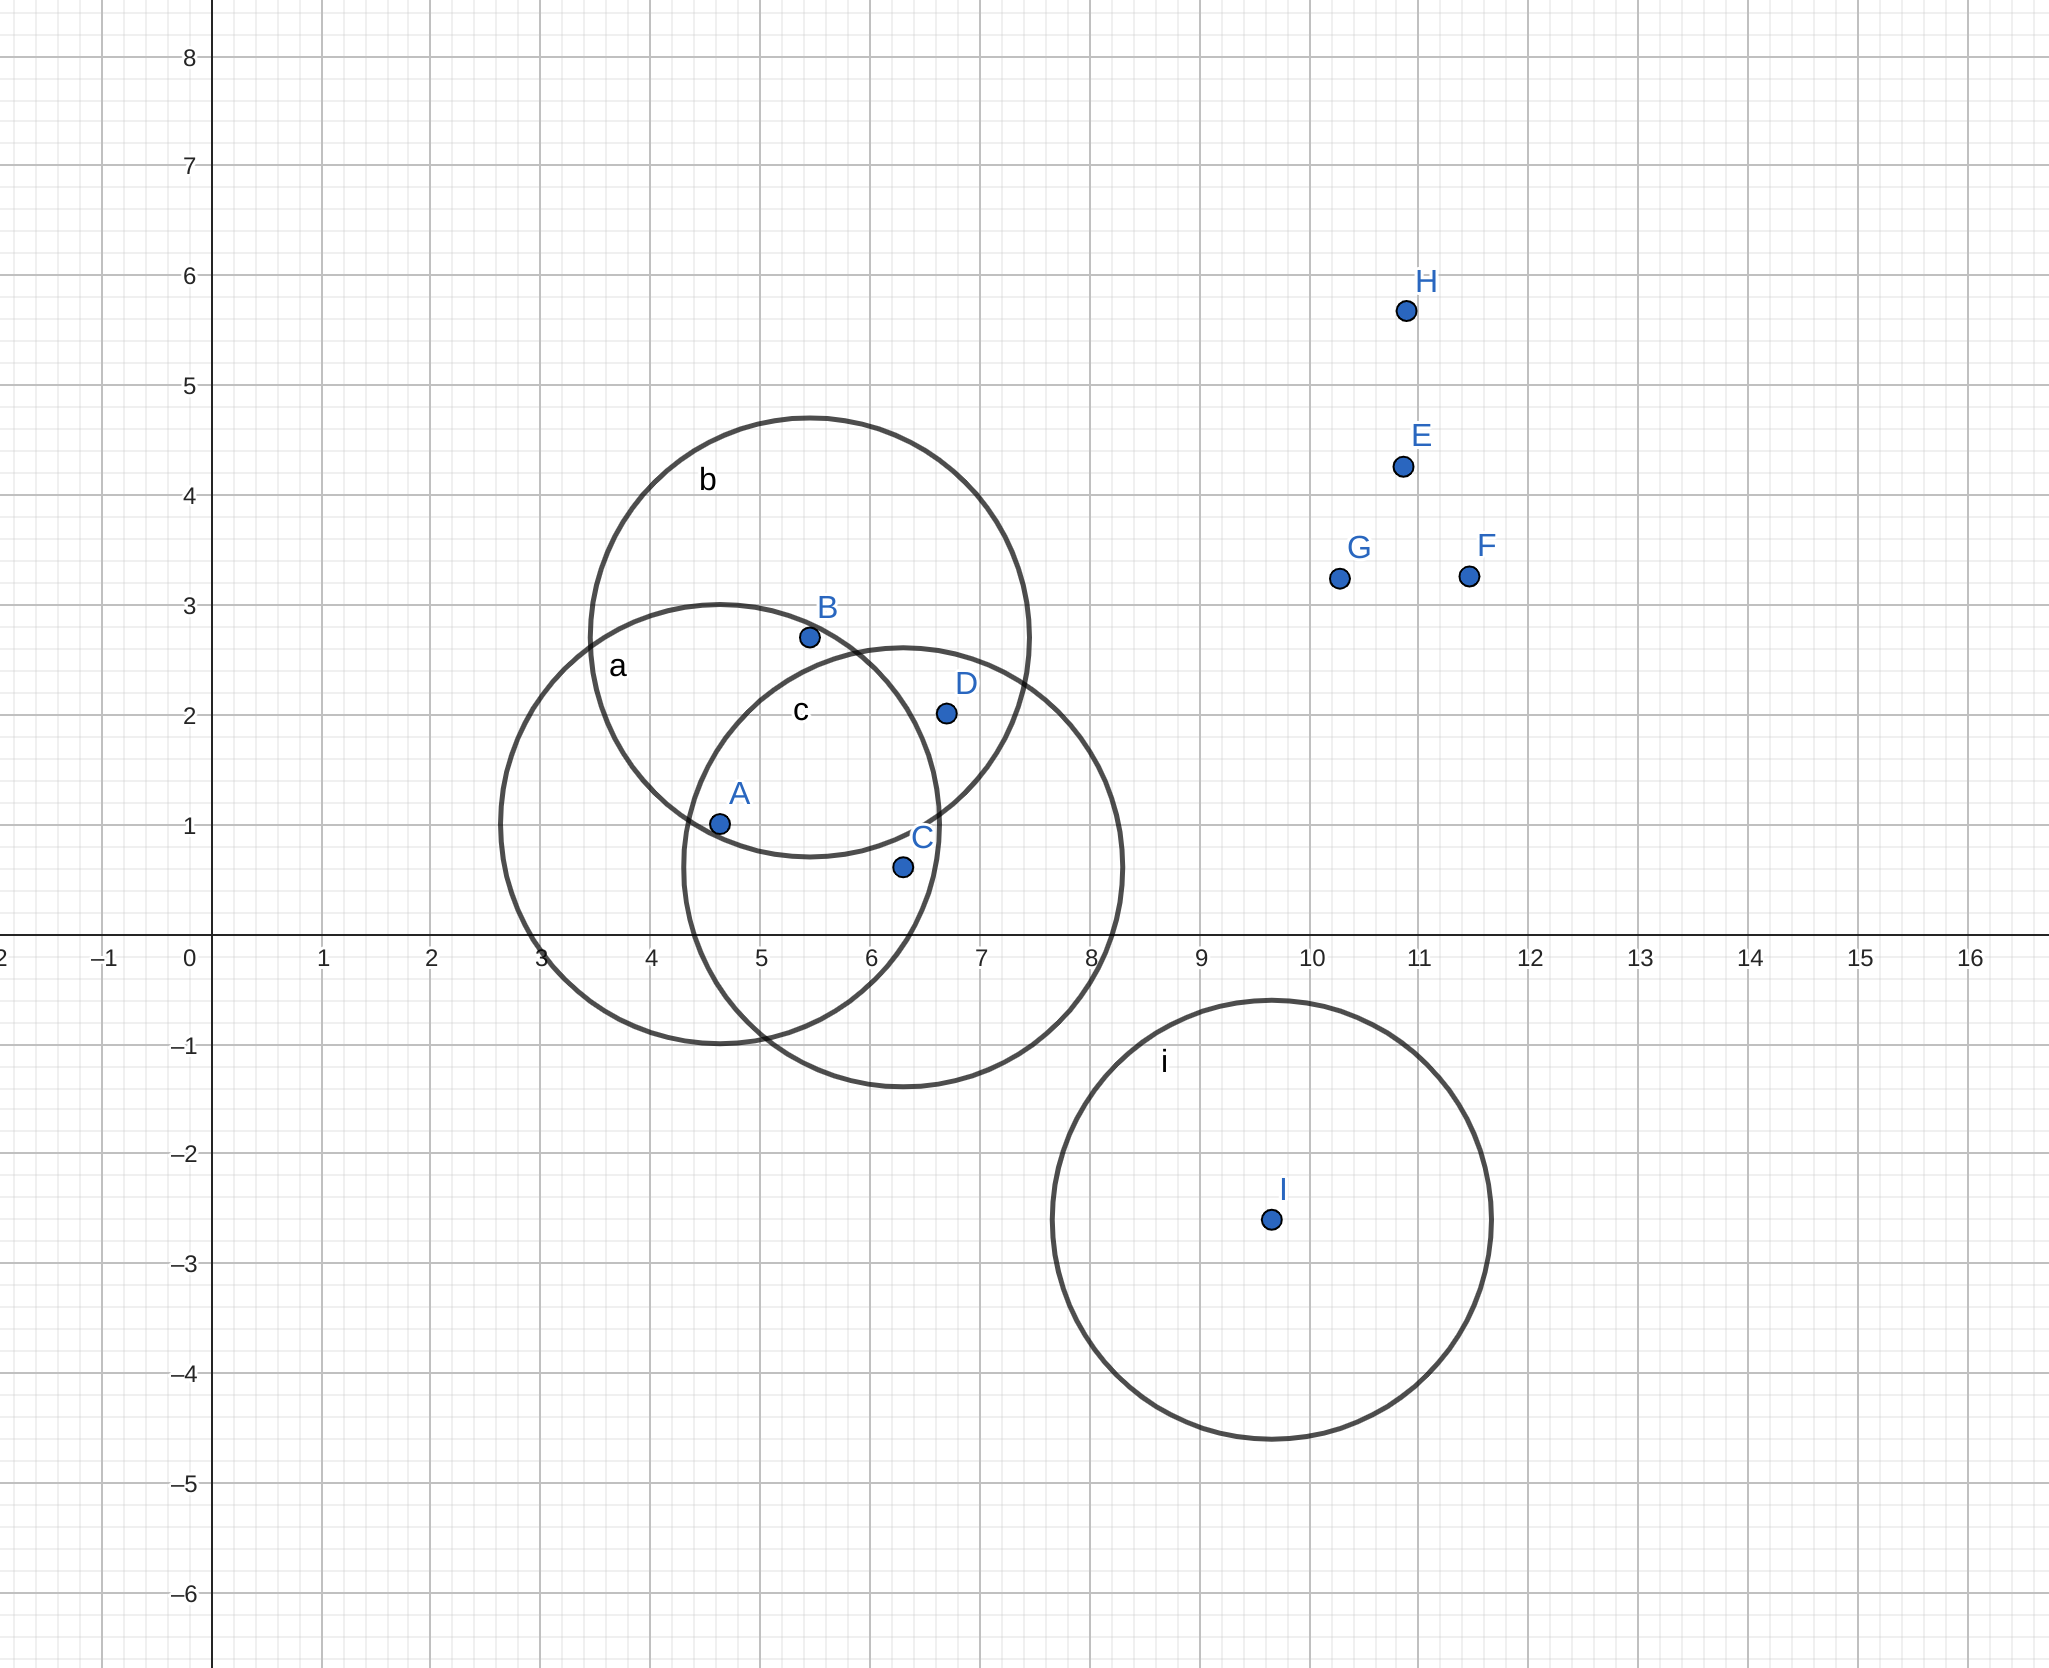
\includegraphics[height=0.41\paperheight]{images/Illustration_DBScan_1.png}
                \caption{\label{fig:ill_DBScan_1} DBScan : Détection des voisins}
            \end{figure}
        \end{column}
    \end{columns}

    \begin{table}[!ht]
        \centering
        \begin{tabular}{c|ccccc}
            \textbf{Point} & \textbf{A} & \textbf{B} & \textbf{C} & \textbf{\dots} & \textbf{I} \\ \hline
            \textbf{N(Points)} & $\left\{ A, B, C \right\}$ & $\left\{ A, B, D \right\}$ & $\left\{ A, C, D \right\}$ & & $\left\{ I \right\}$ \\ 
        \end{tabular}
    \end{table}
\end{frame}

\begin{frame}{Fonctionnement DBScan (2/2)}
    \begin{columns}
        \begin{column}{0.55\textwidth}
            \begin{block}{Etape 2 - Constuction du graphe de voisinage des noyaux}
                \begin{itemize}
                    \item Les points ayant au moins $n_{min}$ voisins sont considérés comme des noyaux. On construit alors un graphe dont les sommets sont les noyaux et il existe une arete entre deux noyaux si et seulement si ils sont voisins.
                    \item Les composantes connexes de ce graphe sont les clusters. On rattache alors aux clusters les points voisins d'au moins un noyau de ce cluster, on les appelle points de bordure.
                    \item Enfin, les sommets qui n'apparaissent pas dans le graphe sont considérés comme du bruit (pas de classe).
                \end{itemize}
            \end{block}
        \end{column}
        \begin{column}{0.45\textwidth}
            \begin{figure}
                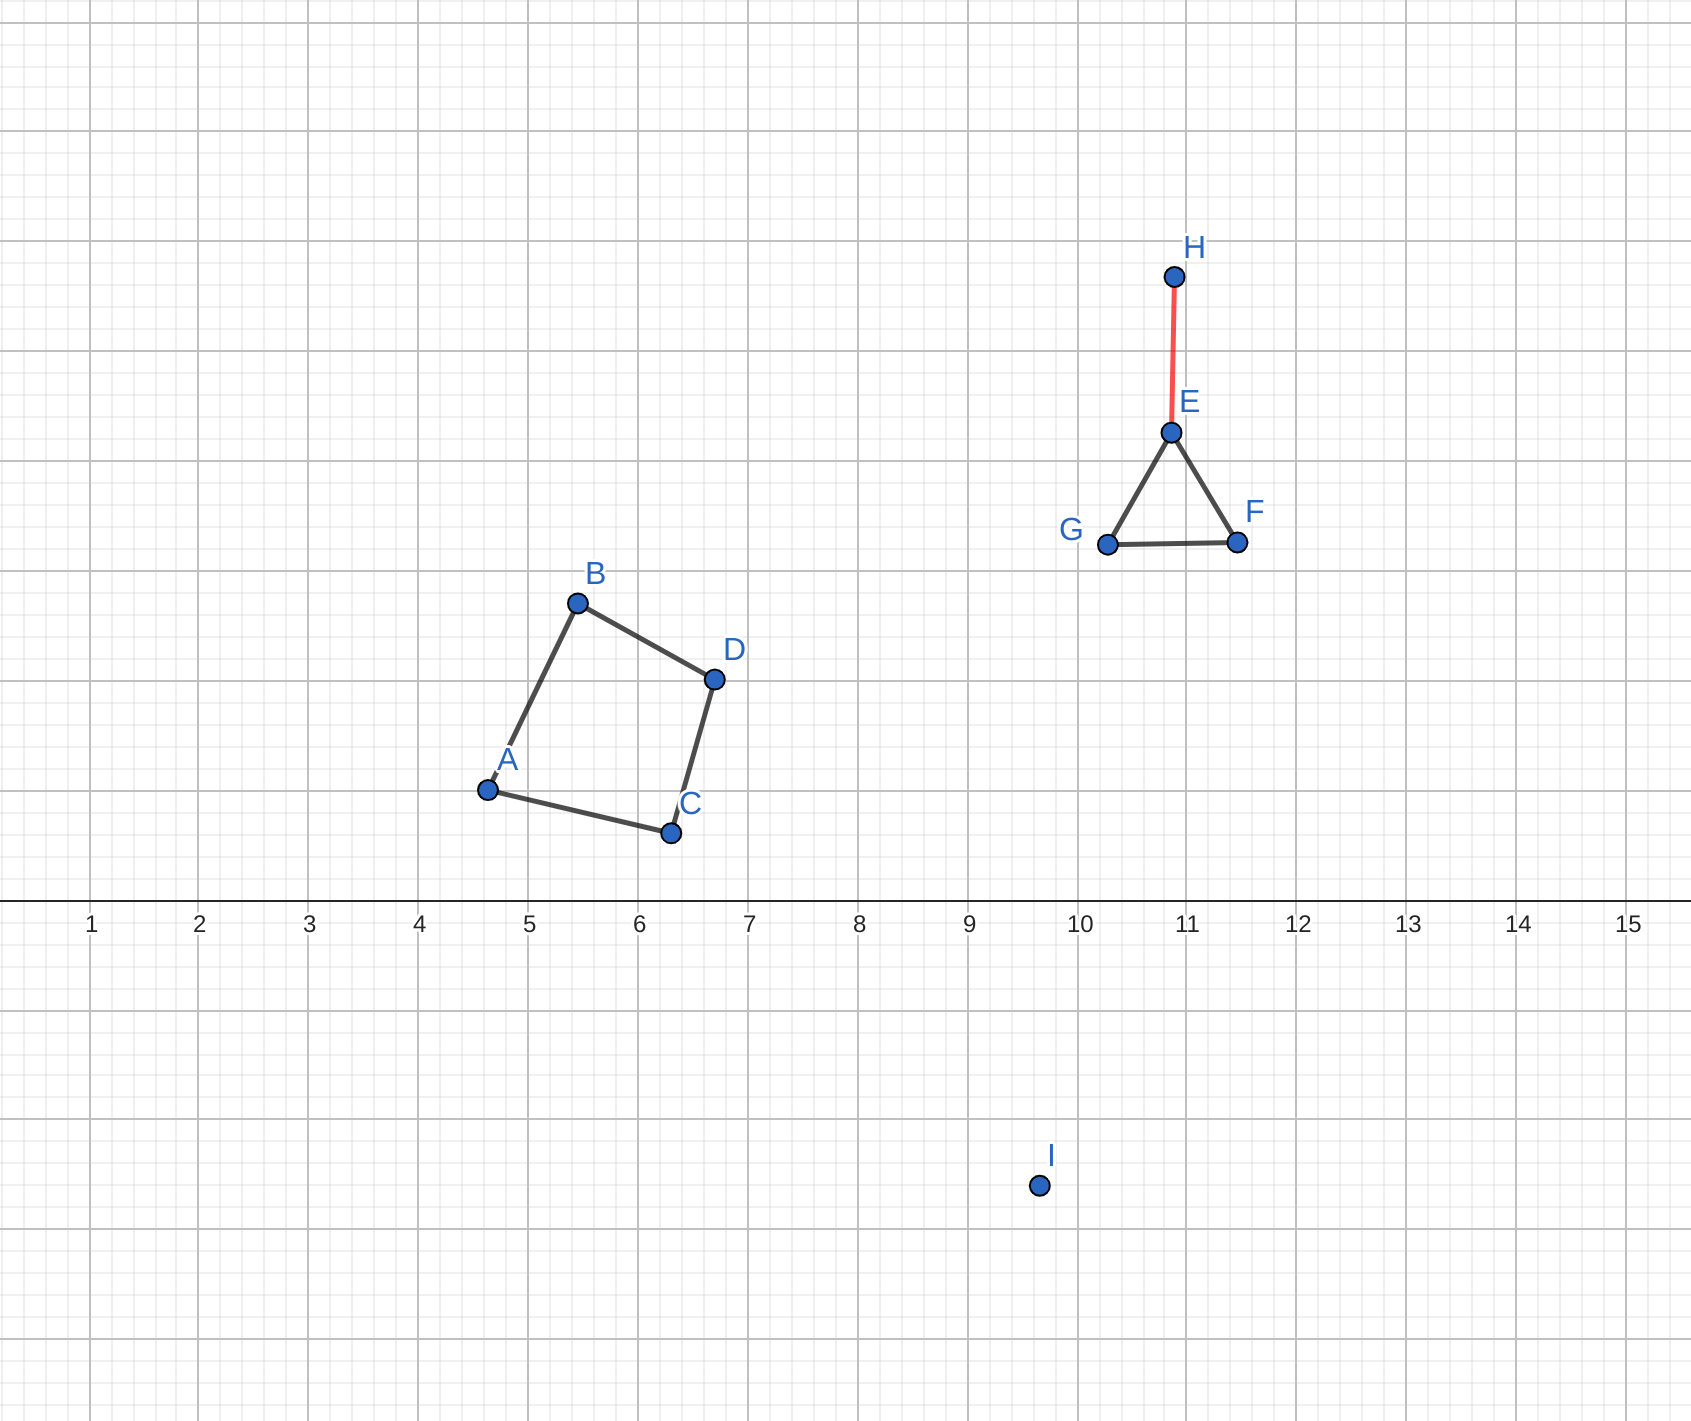
\includegraphics[height=0.5\paperheight]{images/Illustration_DBScan_2.png}
                \caption{\label{fig:ill_DBScan_2} DBScan : création des clusters}
            \end{figure}
        \end{column}
    \end{columns}
\end{frame}

\begin{frame}{Changement de métrique}
    Une façon d'améliorer le problème de mauvaise prise en compte du bruit est de changer de métrique :
    \begin{columns}
        \begin{column}{0.55\textwidth}
            \begin{block}{\emph{Core distance}}
                La \emph{core distance} d'un point du jeu de donnée est la distance entre ce point et son $k$-ième plus proche point ($k$ à fixer).
            \end{block}
        
            \begin{block}{Nouvelle métrique}
                La distance entre deux points $x$ et $y$ d'un jeu de donnée peut être définie comme la plus grande valeur entre les \emph{core distances} de $x$ et $y$ et la distance eucliedienne entre $x$ et $y$.
            \end{block}
        \end{column}
        \begin{column}{0.4\textwidth}
            \begin{figure}
                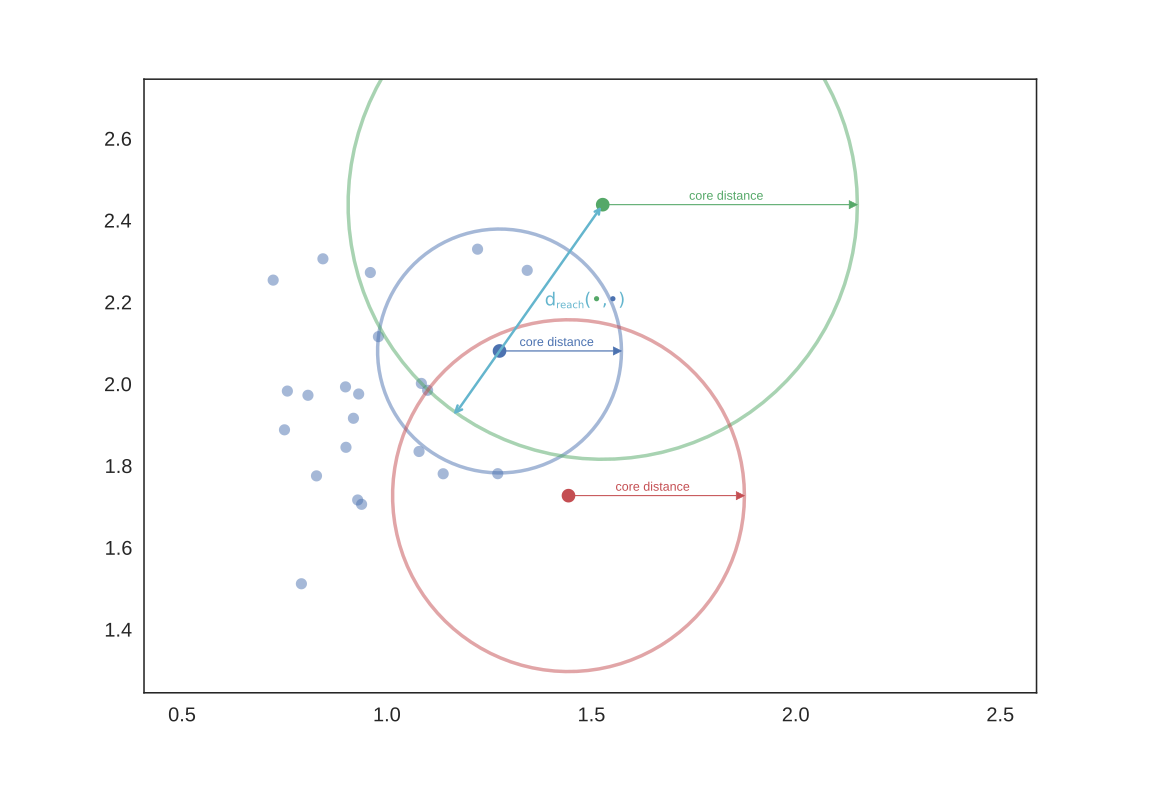
\includegraphics[width=0.6\paperheight]{images/metrique.png}
                \caption{\label{fig:metrique}Nouvelle métrique}
            \end{figure}
        \end{column}
    \end{columns}
\end{frame}



\begin{frame}{Fonctionnement HDBScan\footnotemark }
    \begin{block}{Principe général}
        HDBScan consiste à fusionner les méthodes de classification hierarchique adscendante et DBScan pour permettre de s'affranchir du paramètre $\varepsilon$.
    \end{block}


    \begin{figure}
        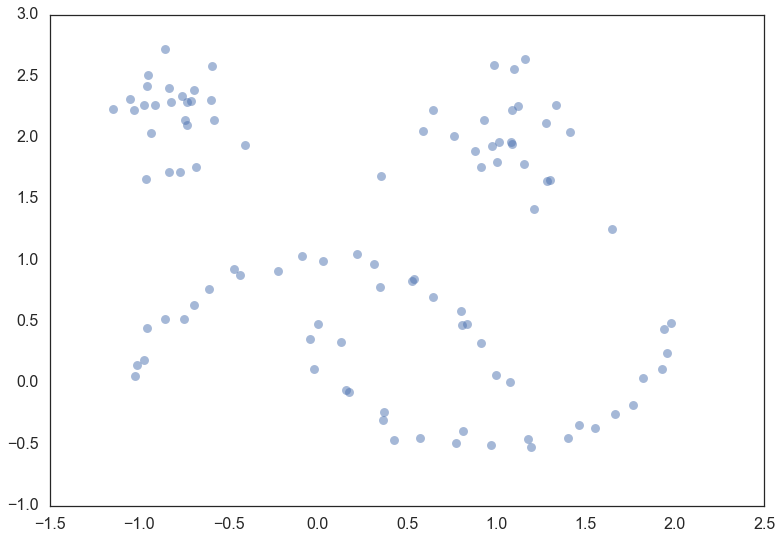
\includegraphics[width=0.5\paperheight]{images/Illustration-HDBSCAN-1.png}
        \caption{\label{fig:ill_HDBScan_1}Le jeu de donnée exemple \footnotemark}
    \end{figure}

    \footnotetext{\url{http://link.springer.com/chapter/10.1007\%2F978-3-642-37456-2\_14}}
    \footnotetext{\url{{https://hdbscan.readthedocs.io/en/latest/how\_hdbscan_works.html}}}
\end{frame}

\begin{frame}{Fonctionnement HDBScan }
    \begin{columns}
        \begin{column}{0.55\textwidth}
            \begin{block}{Etape 1 - Constuction de l'abre couvrant de poids minimum}
                \begin{itemize}
                    \item Représenter les données par un graphe complet où chaque point est un sommet
                    \item Valuer les arêtes par la métrique expliquée précédemment;
                    \item Trouver un arbre couvrant de poids minimum dans ce graphe;
                \end{itemize}
            \end{block}
        \end{column}
        \begin{column}{0.45\textwidth}
            \begin{figure}
                \includegraphics[height=0.4\paperheight]{images/Illustration-HDBScan-2.png}
                \caption{\label{fig:ill_HDBScan_2} Arbre couvrant de poids minimum}
            \end{figure}
        \end{column}
    \end{columns}
\end{frame}

\begin{frame}{Fonctionnement HDBScan }
    \begin{columns}
        \begin{column}{0.55\textwidth}
            \begin{block}{Etape 2 - Création du dendrogramme}
                \begin{itemize}
                    \item Ne garder que les arêtes correspondant à un certain seuil que l'on fait varier.
                    \item Observer l'évolution des classes (composantes connexes) en fonction de cette distance.
                    \item Construire un dendrogramme à partir de ces informations.
                \end{itemize}
            \end{block}
        \end{column}
        \begin{column}{0.45\textwidth}
            \begin{figure}
                \includegraphics[height=0.4\paperheight]{images/Illustration-HDBScan-3.png}
                \caption{\label{fig:ill_HDBScan_3} Dendrogramme}
            \end{figure}
        \end{column}
    \end{columns}
\end{frame}

\begin{frame}{Fonctionnement HDBScan }
    \begin{columns}
        \begin{column}{0.55\textwidth}
            \begin{block}{Etape 3 - Condensation du dendrogramme}
                    On va chercher à condenser le dendrogramme précédent. Pour cela, on considère qu'au départ il n'y a qu'un cluster.
                    On considère qu'un cluster n'est plus considéré comme tel quand il possède moins d'individu qu'un certain seuil (appelons le $n_{min}$).
                    A chaque séparation dans le dendrogramme, il y'a trois cas de figure :
                    \begin{itemize}
                        \item Si les deux parties comportent au moins $n_{min}$ individus, alors on considère que le cluster parent meurt et donne naissance à deux enfants.
                        \item Si une seule des parties comporte au moins $n_{min}$ individus, alors on considère que ce cluster est la continuation du précédent.
                        \item Si les deux parties comportent moins de $n_{min}$ individus, alors on considère que le cluster meurt.
                    \end{itemize}

            \end{block}
        \end{column}
        \begin{column}{0.45\textwidth}
            \begin{figure}
                \includegraphics[height=0.4\paperheight]{images/Illustration-HDBScan-4.png}
                \caption{\label{fig:ill_HDBScan_4} Dendrogramme condensé}
            \end{figure}
        \end{column}
    \end{columns}
\end{frame}

\begin{frame}{Fonctionnement HDBScan }
    \begin{columns}
        \begin{column}{0.55\textwidth}
            \begin{block}{Etape 4 - Selection des clusters}
                    On va choisir les clusters que l'on veut grader au sein du dendrogramme condensé en choisissant les clusters les plus "durables".
                    Graphiquement, cela revient à choisir les clusters dont l'aire est la plus importante dans le dendrogramme condensé.
                    A la fin on souhaite une partition, donc qu'on ne peut selectionner à la fois un cluster et son descendant.
            \end{block}
        \end{column}
        \begin{column}{0.45\textwidth}
            \begin{figure}
                \includegraphics[height=0.4\paperheight]{images/Illustration-HDBScan-5.png}
                \caption{\label{fig:ill_HDBScan_5} Clusters choisis}
            \end{figure}
        \end{column}
    \end{columns}
\end{frame}

\begin{frame}{Fonctionnement HDBScan }
    \begin{columns}
        \begin{column}{0.55\textwidth}
            \begin{block}{Etape 5 - Resultat}
                    A la fin, on obtient les clusters ainsi qu'une probabilité pour chaque point qui caractèrise la probabilité que le point appartienne à son cluster. Cette probabilité est déterminée en observant à quel moment le point se déconnecte de son cluster dans le dengdrogramme.
            \end{block}
        \end{column}
        \begin{column}{0.45\textwidth}
            \begin{figure}
                \includegraphics[height=0.4\paperheight]{images/Illustration-HDBScan-6.png}
                \caption{\label{fig:ill_HDBScan_6} Résulats sur le jeu de donnée d'exemple}
            \end{figure}
        \end{column}
    \end{columns}
\end{frame}


\begin{frame}{HDBScan}
    \begin{block}{Avantages}
        \begin{itemize}
            \item Permet de prendre en compte les probèmes de classe à densité variable;
            \item Introduit un modèle probabiliste.
        \end{itemize}
    \end{block}

    \begin{block}{Application à notre cas d'utilisation}
        \begin{itemize}
            \item Appliqué de la même manière que DBScan : si un point est dans un cluster, alors on considère qu'il est en ville, sinon en campagne;
            \item La probabilité discutée précédemment permet de rajouter une incertitude sur l'appartenance (ou non) d'une station de base à une ville.
        \end{itemize}
    \end{block}
\end{frame}

\begin{frame}{Paramètres de sklearn.cluster.HDBSCAN \footnotemark}
    \begin{itemize}
        \item \texttt{min\_cluster\_size=5} : groupings smaller than this size will be left as noise;
        \item \texttt{min\_samples=None} : The number of samples in a neighborhood for a point to be considered as a core point;
        \item \texttt{cluster\_selection\_epsilon=0.0} : Clusters below this value will be merged;
        \item \texttt{max\_cluster\_size=None};
        \item \texttt{metric='euclidean'};
        \item \texttt{metric\_params=None};
        \item \texttt{alpha=1.0} : A distance scaling parameter;
        \item \texttt{algorithm='auto'} : Exactly which algorithm to use for computing core distances;
        \item \texttt{leaf\_size=40} : Leaf size for trees responsible for fast nearest neighbour queries when a KDTree or a BallTree are used as core-distance algorithms;
        \item \texttt{n\_jobs=None} : Number of jobs to run in parallel to calculate distances;
        \item \texttt{cluster\_selection\_method='eom'} : The method used to select clusters from the condensed tree;
        \item \texttt{allow\_single\_cluster=False} : allow the result to be a single cluster;
        \item \texttt{store\_centers=None};
        \item \texttt{copy=False}.
    \end{itemize}
    \footnotetext{\url{https://scikit-learn.org/stable/modules/generated/sklearn.cluster.HDBSCAN.html}}
\end{frame}

\begin{frame}{Résultats}
    \begin{figure}
        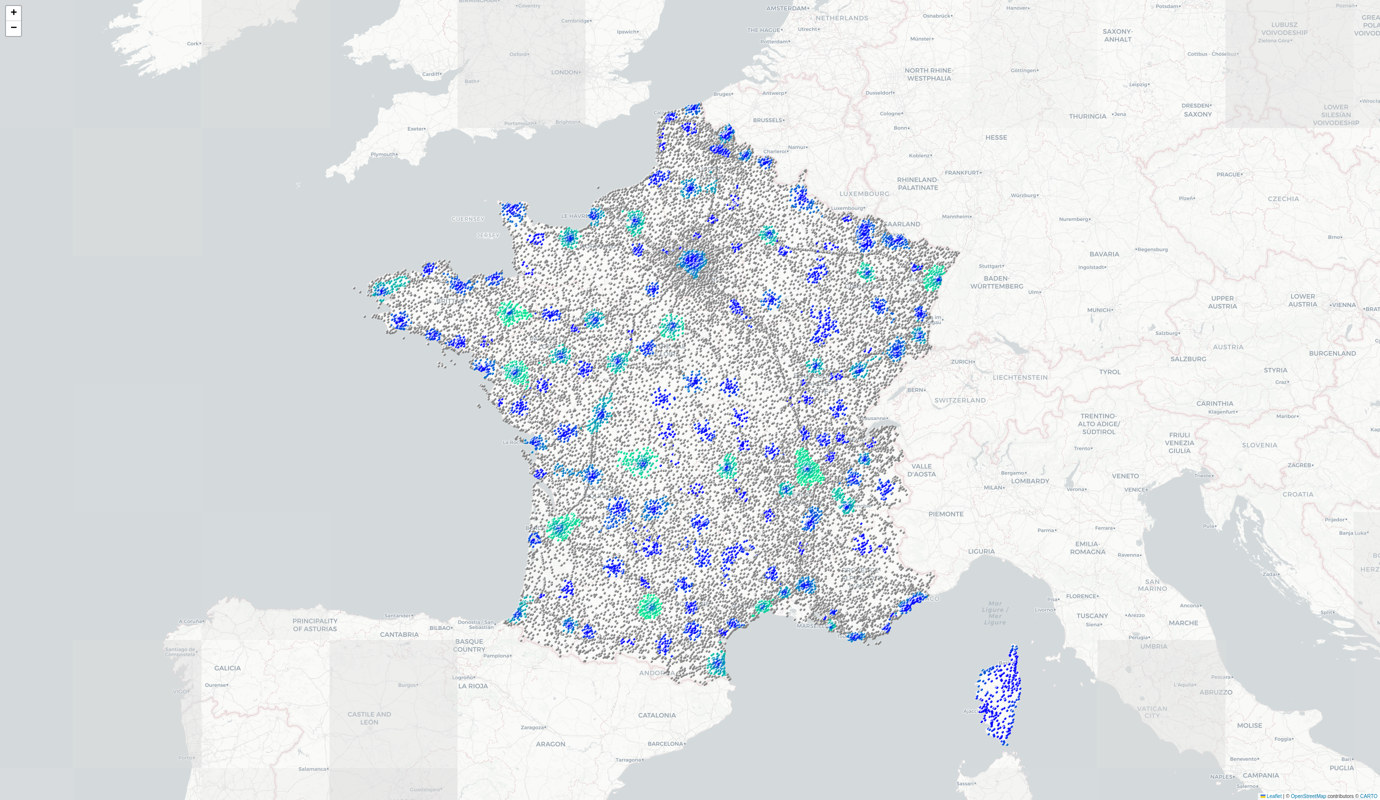
\includegraphics[width=0.9\paperheight]{images/villes_HDBSCAN.png}
        \caption{\label{fig:HDBSCAN}Application d'HDBScan \texttt{min\_cluster\_size=5}, \texttt{min\_samples=40}}
    \end{figure}
\end{frame}





\end{document}
